%debug
%\documentclass[11pt,reqno]{book}

\documentclass[11pt,reqno,oneside]{book}
%debug fim

%---------------------------------------------------------------------
%	VARIOUS REQUIRED PACKAGES AND CONFIGURATIONS
%---------------------------------------------------------------------

\usepackage{comment}
\usepackage{graphicx} % Required for including pictures
\graphicspath{{Pictures/}} 
\usepackage{lipsum} % Inserts dummy text

% Required for drawing custom shapes
\usepackage{tikz} 
\usetikzlibrary{shadows}
\usetikzlibrary{fadings}
\usepackage{tcolorbox}
\tcbuselibrary{skins}
\definecolor{mygreen}{RGB}{0, 128, 0}
\usepackage{subfigure}
\usepackage{float}

\usepackage[portuguese]{babel} % English language/hyphenation
\usepackage{enumitem} % Customize lists
\setlist{nolistsep} 
\usepackage{booktabs} % Required for nicer horizontal rules in tables
\usepackage{xcolor} % Required for specifying colors by name
\definecolor{ocre}{HTML}{1E3543} 
\definecolor{chapterheadazul}{HTML}{1E3543}
\definecolor{chapterhead}{HTML}{ffffff} 
\usepackage{sectsty} %CHange Color for Headings
\usepackage{indentfirst}
\usepackage{graphicx,wrapfig}
\usepackage[pt-BR]{datetime2}


%---------------------------------------------------------------------
%	MARGINS
%---------------------------------------------------------------------

\usepackage{geometry} % Required for adjusting page dimensions and margins

\geometry{
	paper=a4paper, % Paper size, change to letterpaper for US letter size
	top=3cm, % Top margin
	bottom=2cm, % Bottom margin
	left=3cm, % Left margin
	right=2cm, % Right margin
	headheight=14pt, % Header height
	footskip=1.4cm, % Space from the bottom margin to the baseline of the footer
	headsep=10pt, % Space from the top margin to the baseline of the header
}

%---------------------------------------------------------------------
%	FONTS
%---------------------------------------------------------------------

\usepackage{avant} % Use the Avantgarde font for headings
%\usepackage{times} % Use the Times font for headings
\usepackage{mathptmx} % Use the Adobe Times Roman as the default text font together with math symbols from the Sym­bol, Chancery and Com­puter Modern fonts

\usepackage{microtype} % Slightly tweak font spacing for aesthetics
\usepackage[utf8]{inputenc} % Required for including letters with accents
\usepackage[T1]{fontenc} % Use 8-bit encoding that has 256 glyphs
\usepackage{setspace}
\usepackage{csquotes}

%---------------------------------------------------------------------
%	BIBLIOGRAPHY AND INDEX
%---------------------------------------------------------------------

\usepackage[style=numeric,citestyle=numeric,sorting=nyt,sortcites=true,autopunct=true,hyperref=true,abbreviate=false,backref=true,backend=biber]{biblatex}
\addbibresource{bibliography.bib} % BibTeX bibliography file
\defbibheading{bibempty}{}

\usepackage{calc} % For simpler calculation - used for spacing the index letter headings correctly
\usepackage{makeidx} % Required to make an index
\makeindex % Tells LaTeX to create the files required for indexing

%---------------------------------------------------------------------
%	MAIN TABLE OF CONTENTS
%---------------------------------------------------------------------

\usepackage{titletoc} % Required for manipulating the table of contents

\contentsmargin{0cm} % Removes the default margin

% Part text styling (this is mostly taken care of in the PART HEADINGS section of this file)
\titlecontents{part}
	[0cm] % Left indentation
	{\addvspace{20pt}\bfseries} % Spacing and font options for parts
	{}
	{}
	{}

% Chapter text styling
\titlecontents{chapter}
	[1.25cm] % Left indentation
	{\addvspace{12pt}\large\sffamily\bfseries} % Spacing and font options for chapters
	{\color{ocre}\contentslabel[\Large\thecontentslabel]{1.25cm}\color{ocre}} % Formatting of numbered sections of this type
	{\color{ocre}} % Formatting of numberless sections of this type
	{\color{ocre}\normalsize\;\titlerule*[.5pc]{.}\;\thecontentspage} % Formatting of the filler to the right of the heading and the page number

% Section text styling
\titlecontents{section}
	[1.25cm] % Left indentation
	{\addvspace{3pt}\sffamily\bfseries} % Spacing and font options for sections
	{\contentslabel[\thecontentslabel]{1.25cm}} % Formatting of numbered sections of this type
	{} % Formatting of numberless sections of this type
	{\hfill\color{black}\thecontentspage} % Formatting of the filler to the right of the heading and the page number

% Subsection text styling
\titlecontents{subsection}
	[1.25cm] % Left indentation
	{\addvspace{1pt}\sffamily\small} % Spacing and font options for subsections
	{\contentslabel[\thecontentslabel]{1.25cm}} % Formatting of numbered sections of this type
	{} % Formatting of numberless sections of this type
	{\ \titlerule*[.5pc]{.}\;\thecontentspage} % Formatting of the filler to the right of the heading and the page number

% Figure text styling
\titlecontents{figure}
	[1.25cm] % Left indentation
	{\addvspace{1pt}\sffamily\small} % Spacing and font options for figures
	{\thecontentslabel\hspace*{1em}} % Formatting of numbered sections of this type
	{} % Formatting of numberless sections of this type
	{\ \titlerule*[.5pc]{.}\;\thecontentspage} % Formatting of the filler to the right of the heading and the page number

% Table text styling
\titlecontents{table}
	[1.25cm] % Left indentation
	{\addvspace{1pt}\sffamily\small} % Spacing and font options for tables
	{\thecontentslabel\hspace*{1em}} % Formatting of numbered sections of this type
	{} % Formatting of numberless sections of this type
	{\ \titlerule*[.5pc]{.}\;\thecontentspage} % Formatting of the filler to the right of the heading and the page number

%---------------------------------------------------------------------
%	MINI TABLE OF CONTENTS IN PART HEADS
%---------------------------------------------------------------------

% Chapter text styling
\titlecontents{lchapter}
	[0em] % Left indentation
	{\addvspace{15pt}\large\sffamily\bfseries\color{white}} % Spacing and font options for chapters
	{\color{chapterhead}\contentslabel[\Large\thecontentslabel]{1.25cm}\color{chapterhead}} % Chapter number
	{}  
	{\color{chapterhead}\normalsize\sffamily\bfseries\;\titlerule*[.5pc]{.}\;\thecontentspage} % Page number

% Section text styling
\titlecontents{lsection}
	[0em] % Left indentation
	{\sffamily\small} % Spacing and font options for sections
	{\color{chapterhead}\contentslabel[\thecontentslabel]{1.25cm}} % Section number
	{}
	{}

% Subsection text styling (note these aren't shown by default, display them by searchings this file for tocdepth and reading the commented text)
\titlecontents{lsubsection}
	[.5em] % Left indentation
	{\sffamily\footnotesize} % Spacing and font options for subsections
	{\color{chapterhead}\contentslabel[\thecontentslabel]{1.25cm}}
	{}
	{}

%---------------------------------------------------------------------
%	HEADERS AND FOOTERS
%---------------------------------------------------------------------

\usepackage{fancyhdr} % Required for header and footer configuration

\pagestyle{fancy} % Enable the custom headers and footers

\pagestyle{fancy}
\renewcommand{\chaptermark}[1]{\markboth{\sffamily\normalsize\bfseries\chaptername\ \thechapter.\ #1}{}} % Chapter text font settings
 
\renewcommand{\sectionmark}[1]{\markright{\sffamily\normalsize\thesection\hspace{5pt}#1}{}} % Section text font settings
\fancyhf{} \fancyhead[LE,RO]{\sffamily\normalsize\thepage} % Font setting for the page number in the header
\fancyhead[LO]{\rightmark} % Print the nearest section name on the left side of odd pages
\fancyhead[RE]{\leftmark} % Print the current chapter name on the right side of even pages
\renewcommand{\headrulewidth}{0.5pt} % Width of the rule under the header
\addtolength{\headheight}{2.5pt} % Increase the spacing around the header slightly
\renewcommand{\footrulewidth}{0pt} % Removes the rule in the footer
\fancypagestyle{plain}{\fancyhead{}\renewcommand{\headrulewidth}{0pt}} % Style for when a plain pagestyle is specified

% Removes the header from odd empty pages at the end of chapters
\makeatletter
\renewcommand{\cleardoublepage}{
\clearpage\ifodd\c@page\else
\hbox{}
\vspace*{\fill}
\thispagestyle{empty}
\newpage
\fi}

%---------------------------------------------------------------------
%	THEOREM STYLES
%---------------------------------------------------------------------

\usepackage{amsmath,amsfonts,amssymb,amsthm} % For math equations, theorems, symbols, etc

\newcommand{\intoo}[2]{\mathopen{]}#1\,;#2\mathclose{[}}
\newcommand{\ud}{\mathop{\mathrm{{}d}}\mathopen{}}
\newcommand{\intff}[2]{\mathopen{[}#1\,;#2\mathclose{]}}
\renewcommand{\qedsymbol}{$\blacksquare$}
\newtheorem{notation}{Notação}[chapter]

% Boxed/framed environments
\newtheoremstyle{ocrenumbox}% Theorem style name
{0pt}% Space above
{0pt}% Space below
{\normalfont}% Body font
{}% Indent amount
{\small\bf\sffamily\color{ocre}}% Theorem head font
{\;}% Punctuation after theorem head
{0.25em}% Space after theorem head
{\small\sffamily\color{ocre}\thmname{#1}\nobreakspace\thmnumber{\@ifnotempty{#1}{}\@upn{#2}}% Theorem text (e.g. Theorem 2.1)
\thmnote{\nobreakspace\the\thm@notefont\sffamily\bfseries\color{black}---\nobreakspace#3.}} % Optional theorem note

\newtheoremstyle{blacknumex}% Theorem style name
{5pt}% Space above
{5pt}% Space below
{\normalfont}% Body font
{} % Indent amount
{\small\bf\sffamily}% Theorem head font
{\;}% Punctuation after theorem head
{0.25em}% Space after theorem head
{\small\sffamily{\tiny\ensuremath{\blacksquare}}\nobreakspace\thmname{#1}\nobreakspace\thmnumber{\@ifnotempty{#1}{}\@upn{#2}}% Theorem text (e.g. Theorem 2.1)
\thmnote{\nobreakspace\the\thm@notefont\sffamily\bfseries---\nobreakspace#3.}}% Optional theorem note

\newtheoremstyle{blacknumbox} % Theorem style name
{0pt}% Space above
{0pt}% Space below
{\normalfont}% Body font
{}% Indent amount
{\small\bf\sffamily}% Theorem head font
{\;}% Punctuation after theorem head
{0.25em}% Space after theorem head
{\small\sffamily\thmname{#1}\nobreakspace\thmnumber{\@ifnotempty{#1}{}\@upn{#2}}% Theorem text (e.g. Theorem 2.1)
\thmnote{\nobreakspace\the\thm@notefont\sffamily\bfseries---\nobreakspace#3.}}% Optional theorem note

% Non-boxed/non-framed environments
\newtheoremstyle{ocrenum}% Theorem style name
{5pt}% Space above
{5pt}% Space below
{\normalfont}% Body font
{}% Indent amount
{\small\bf\sffamily\color{ocre}}% Theorem head font
{\;}% Punctuation after theorem head
{0.25em}% Space after theorem head
{\small\sffamily\color{ocre}\thmname{#1}\nobreakspace\thmnumber{\@ifnotempty{#1}{}\@upn{#2}}% Theorem text (e.g. Theorem 2.1)
\thmnote{\nobreakspace\the\thm@notefont\sffamily\bfseries\color{black}---\nobreakspace#3.}} % Optional theorem note
\makeatother

% Defines the theorem text style for each type of theorem to one of the three styles above
\newcounter{dummy} 
\numberwithin{dummy}{section}
\theoremstyle{ocrenumbox}
\newtheorem{theoremeT}[dummy]{Teorema}
\newtheorem{problem}{Problema}[chapter]
\newtheorem{exerciseT}{Exercício}[chapter]
\theoremstyle{blacknumex}
\newtheorem{exampleT}{Exemplo}[chapter]
\theoremstyle{blacknumbox}
\newtheorem{vocabulary}{Vocabulário}[chapter]
\newtheorem{definitionT}{Definição}[section]
\newtheorem{corollaryT}[dummy]{Corolário}
\theoremstyle{ocrenum}
\newtheorem{proposition}[dummy]{Proposição}

%---------------------------------------------------------------------
%	DEFINITION OF COLORED BOXES
%---------------------------------------------------------------------

\RequirePackage[framemethod=default]{mdframed} % Required for creating the theorem, definition, exercise and corollary boxes

% Theorem box
\newmdenv[skipabove=7pt,
skipbelow=7pt,
backgroundcolor=white,
linecolor=ocre,
innerleftmargin=5pt,
innerrightmargin=5pt,
innertopmargin=5pt,
leftmargin=0cm,
rightmargin=0cm,
innerbottommargin=5pt]{tBox}

% Exercise box	  
\newmdenv[skipabove=7pt,
skipbelow=7pt,
rightline=false,
leftline=true,
topline=false,
bottomline=false,
backgroundcolor=white,
linecolor=ocre,
innerleftmargin=5pt,
innerrightmargin=5pt,
innertopmargin=5pt,
innerbottommargin=5pt,
leftmargin=0cm,
rightmargin=0cm,
linewidth=4pt]{eBox}	

% Definition box
\newmdenv[skipabove=7pt,
skipbelow=7pt,
rightline=false,
leftline=true,
topline=false,
bottomline=false,
linecolor=ocre,
innerleftmargin=5pt,
innerrightmargin=5pt,
innertopmargin=0pt,
leftmargin=0cm,
rightmargin=0cm,
linewidth=4pt,
innerbottommargin=0pt]{dBox}	

% Corollary box
\newmdenv[skipabove=7pt,
skipbelow=7pt,
rightline=false,
leftline=true,
topline=false,
bottomline=false,
linecolor=gray,
backgroundcolor=black!5,
innerleftmargin=5pt,
innerrightmargin=5pt,
innertopmargin=5pt,
leftmargin=0cm,
rightmargin=0cm,
linewidth=4pt,
innerbottommargin=5pt]{cBox}

% Creates an environment for each type of theorem and assigns it a theorem text style from the "Theorem Styles" section above and a colored box from above
\newenvironment{theorem}{\begin{tBox}\begin{theoremeT}}{\end{theoremeT}\end{tBox}}
\newenvironment{exercise}{\begin{eBox}\begin{exerciseT}}{\hfill{\color{ocre}\tiny\ensuremath{\blacksquare}}\end{exerciseT}\end{eBox}}				  
\newenvironment{definition}{\begin{dBox}\begin{definitionT}}{\end{definitionT}\end{dBox}}	
\newenvironment{example}{\begin{exampleT}}{\hfill{\tiny\ensuremath{\blacksquare}}\end{exampleT}}		
\newenvironment{corollary}{\begin{cBox}\begin{corollaryT}}{\end{corollaryT}\end{cBox}}	

%---------------------------------------------------------------------
%	REMARK ENVIRONMENT
%---------------------------------------------------------------------

\newenvironment{remark}{\par\vspace{10pt}\small % Vertical white space above the remark and smaller font size
\begin{list}{}{
\leftmargin=35pt % Indentation on the left
\rightmargin=25pt}\item\ignorespaces % Indentation on the right
\makebox[-2.5pt]{\begin{tikzpicture}[overlay]
\node[draw=ocre,line width=1pt,circle,fill=ocre,font=\sffamily\bfseries,inner sep=2pt,outer sep=0pt] at (-15pt,0pt){\textcolor{ocre}{R}};\end{tikzpicture}} % Orange R in a circle
\advance\baselineskip -1pt}{\end{list}\vskip5pt} % Tighter line spacing and white space after remark

%---------------------------------------------------------------------
%	SECTION NUMBERING IN THE MARGIN
%---------------------------------------------------------------------

\makeatletter
\renewcommand{\@seccntformat}[1]{\llap{\textcolor{ocre}{\csname the#1\endcsname}\hspace{1em}}}                    
\renewcommand{\section}{\@startsection{section}{1}{\z@}
{-4ex \@plus -1ex \@minus -.4ex}
{1ex \@plus.2ex }
{\normalfont\large\sffamily\bfseries}}
\renewcommand{\subsection}{\@startsection {subsection}{2}{\z@}
{-3ex \@plus -0.1ex \@minus -.4ex}
{0.5ex \@plus.2ex }
{\normalfont\sffamily\bfseries}}
\renewcommand{\subsubsection}{\@startsection {subsubsection}{3}{\z@}
{-2ex \@plus -0.1ex \@minus -.2ex}
{.2ex \@plus.2ex }
{\normalfont\small\sffamily\bfseries}}                        
\renewcommand\paragraph{\@startsection{paragraph}{4}{\z@}
{-2ex \@plus-.2ex \@minus .2ex}
{.1ex}
{\normalfont\small\sffamily\bfseries}}

%---------------------------------------------------------------------
%	PART HEADINGS
%---------------------------------------------------------------------

% Numbered part in the table of contents
\newcommand{\@mypartnumtocformat}[2]{%
	\setlength\fboxsep{0pt}%
	\noindent\colorbox{ocre}{\strut\parbox[c][.7cm]{\ecart}{\color{ocre}\Large\sffamily\bfseries\centering\color{chapterhead}#1}}\hskip\esp\colorbox{ocre}{\strut\parbox[c][.7cm]{\linewidth-\ecart-\esp}{\Large\sffamily\centering\color{chapterhead}#2}}%
}

% Unnumbered part in the table of contents
\newcommand{\@myparttocformat}[1]{%
	\setlength\fboxsep{0pt}\color{ocre}%
	\noindent\colorbox{ocre}{\strut\parbox[c][.7cm]{\linewidth}{\Large\sffamily\centering\color{ocre}#1}}%
}

\newlength\esp
\setlength\esp{4pt}
\newlength\ecart
\setlength\ecart{1.2cm-\esp}
\newcommand{\thepartimage}{}%
\newcommand{\partimage}[1]{\renewcommand{\color{ocre}\thepartimage}{#1}}%
\def\@part[#1]#2{%
\ifnum \c@secnumdepth >-2\relax%
\refstepcounter{part}%
\addcontentsline{toc}{part}{\texorpdfstring{\protect\@mypartnumtocformat{\thepart}{#1}}{\partname~\thepart\ ---\ #1}}
\else%
\addcontentsline{toc}{part}{\texorpdfstring{\protect\@myparttocformat{#1}}{#1}}%
\fi%
\startcontents%
\markboth{}{}%
{\thispagestyle{empty}%
\begin{tikzpicture}[remember picture,overlay]%
\node at (current page.north west){\begin{tikzpicture}[remember picture,overlay]%	
\fill[ocre](0cm,0cm) rectangle (\paperwidth,-\paperheight);
\node[anchor=north] at (4cm,-3.25cm){\color{chapterhead}\fontsize{220}{100}\sffamily\bfseries\thepart}; 
\node[anchor=south east] at (\paperwidth-1cm,-\paperheight+1cm){\parbox[t][][t]{8.5cm}{
\printcontents{l}{0}{\setcounter{tocdepth}{1}}% The depth to which the Part mini table of contents displays headings; 0 for chapters only, 1 for chapters and sections and 2 for chapters, sections and subsections
}};
\node[anchor=north east] at (\paperwidth-1.5cm,-3.25cm){\parbox[t][][t]{15cm}{\strut\raggedleft\color{chapterhead}\fontsize{30}{30}\sffamily\bfseries#2}};
\end{tikzpicture}};
\end{tikzpicture}}%
\@endpart}
\def\@spart#1{%
\startcontents%
\phantomsection
{\thispagestyle{empty}%
\begin{tikzpicture}[remember picture,overlay]%
\node at (current page.north west){\begin{tikzpicture}[remember picture,overlay]%	
\fill[chapterhead](0cm,0cm) rectangle (\paperwidth,-\paperheight);
\node[anchor=north east] at (\paperwidth-1.5cm,-3.25cm){\parbox[t][][t]{15cm}{\strut\raggedleft\color{chapterhead}\fontsize{30}{30}\sffamily\bfseries#1}};
\end{tikzpicture}};
\end{tikzpicture}}
\addcontentsline{toc}{part}{\texorpdfstring{%
\setlength\fboxsep{0pt}%
\noindent\protect\colorbox{ocre}{\strut\protect\parbox[c][.7cm]{\linewidth}{\Large\sffamily\protect\centering #1\quad\mbox{}}}}{#1}}%
\@endpart}
\def\@endpart{\vfil\newpage
\if@twoside
\if@openright
\null
\thispagestyle{empty}%
\newpage
\fi
\fi
\if@tempswa
\twocolumn
\fi}

%---------------------------------------------------------------------
%	CHAPTER HEADINGS
%---------------------------------------------------------------------

% A switch to conditionally include a picture, implemented by Christian Hupfer
\newif\ifusechapterimage
\usechapterimagetrue
\newcommand{\thechapterimage}{}%
\newcommand{\chapterimage}[1]{\ifusechapterimage\renewcommand{\thechapterimage}{#1}\fi}%
\newcommand{\autodot}{.}
\def\@makechapterhead#1{%
{\parindent \z@ \raggedright \normalfont
\ifnum \c@secnumdepth >\m@ne
\if@mainmatter
\begin{tikzpicture}[remember picture,overlay]
\node at (current page.north west)
{\begin{tikzpicture}[remember picture,overlay]
\node[anchor=north west,inner sep=0pt] at (0,0) {\ifusechapterimage\includegraphics[width=\paperwidth]{\thechapterimage}\fi};
\draw[anchor=west] (\Gm@lmargin,-5cm) node [line width=2pt,rounded corners=15pt,draw=ocre,fill=ocre,fill opacity=0.95,inner sep=15pt]{\strut\makebox[22cm]{}};
\draw[anchor=west] (\Gm@lmargin+.3cm,-5cm) node {\huge\sffamily\bfseries\color{chapterhead}\thechapter\autodot~#1\strut};
\end{tikzpicture}};
\end{tikzpicture}
\else
\begin{tikzpicture}[remember picture,overlay]
\node at (current page.north west)
{\begin{tikzpicture}[remember picture,overlay]
\node[anchor=north west,inner sep=0pt] at (0,0) {\ifusechapterimage\includegraphics[width=\paperwidth]{\thechapterimage}\fi};
\draw[anchor=west] (\Gm@lmargin,-5cm) node [line width=2pt,rounded corners=15pt,draw=ocre,fill=white,fill opacity=0.95,inner sep=15pt]{\strut\makebox[22cm]{}};
\draw[anchor=west] (\Gm@lmargin+.3cm,-5cm) node {\huge\sffamily\bfseries\color{black}#1\strut};
\end{tikzpicture}};
\end{tikzpicture}
\fi\fi\par\vspace*{170\p@}}}

%-------------------------------------------

\def\@makeschapterhead#1{%
\begin{tikzpicture}[remember picture,overlay]
\node at (current page.north west)
{\begin{tikzpicture}[remember picture,overlay]
\node[anchor=north west,inner sep=0pt] at (0,0) {\ifusechapterimage\includegraphics[width=\paperwidth]{\thechapterimage}\fi};
\draw[anchor=west] (\Gm@lmargin,-5cm) node [line width=2pt,rounded corners=15pt,draw=ocre,fill=ocre,fill opacity=0.95,inner sep=15pt]{\strut\makebox[22cm]{}};
\draw[anchor=west] (\Gm@lmargin+.3cm,-5cm) node {\huge\sffamily\bfseries\color{chapterhead}#1\strut};
\end{tikzpicture}};
\end{tikzpicture}
\par\vspace*{170\p@}}
\makeatother

%---------------------------------------------------------------------
%	LINKS
%---------------------------------------------------------------------

\usepackage{hyperref}
\hypersetup{hidelinks,backref=true,pagebackref=true,hyperindex=true,colorlinks=false,breaklinks=true,urlcolor=ocre,bookmarks=true,bookmarksopen=false,pdftitle={Apostila Didática},pdfauthor={IFBaiano-Lapa}}

\usepackage{bookmark}
\bookmarksetup{
open,
numbered,
addtohook={%
\ifnum\bookmarkget{level}=0 % chapter
\bookmarksetup{color=ocre, bold}%
\fi
\ifnum\bookmarkget{level}=-1 % part
\bookmarksetup{color=ocre,bold}%
\fi
}
}



%---------------------------------------------------------------------
%	MEUS AMBIENTES
%---------------------------------------------------------------------



\newcommand{\mytitle}[1]{
    \node[left=210pt]
    at (frame.north){#1};
}

\newtcolorbox{mybox}[2][]{
    enhanced,
    overlay={\mytitle{#2}},
    borderline={2pt}{0mm}{mygreen},
    borderline={.7pt}{1mm}{mygreen},
    frame hidden,
    arc=3mm,
    sidebyside,
    lefthand width=2.5cm,
    segmentation hidden,
    top=15pt,
    left=-90pt,
    #1
}


% ATENÇÃO %

\newenvironment{aten}{\par\vspace{0pt}\small
\begin{list}{}{
\leftmargin=-15pt
\rightmargin=25pt}\item\ignorespaces 
\advance\baselineskip -1pt}{\end{list}\vskip5pt} 

\newcommand{\atencao}[1]{
\vspace{0.5cm} \begin{mybox}{\makebox[-2.5pt]{\begin{tikzpicture}[overlay]
\node at (0pt,0pt){
\includegraphics[scale=.6]{atencao}};\end{tikzpicture}}}{\begin{aten}\end{aten}}
    \tcblower
    #1
    \vspace{0.2cm}
\end{mybox}}



% SAIBA MAIS %
\newcommand{\mais}[1]{
\vspace{0.5cm} \begin{mybox}{\makebox[-2.5pt]{\begin{tikzpicture}[overlay]
\node at (0pt,0pt){
\includegraphics[scale=.6]{mais}};\end{tikzpicture}}}{\begin{aten}\end{aten}}
    \tcblower
    #1
    \vspace{0.2cm}
\end{mybox}}

% GLOSSÁRIO %
\newcommand{\glossario}[1]{
\vspace{0.5cm} \begin{mybox}{\makebox[-2.5pt]{\begin{tikzpicture}[overlay]
\node at (0pt,0pt){
\includegraphics[scale=.6]{glossario}};\end{tikzpicture}}}{\begin{aten}\end{aten}}
    \tcblower
    #1
    \vspace{0.2cm}
\end{mybox}}


% MULTIMIDIA %
\newcommand{\midia}[1]{
\vspace{0.5cm} \begin{mybox}{\makebox[-2.5pt]{\begin{tikzpicture}[overlay]
\node at (0pt,0pt){
\includegraphics[scale=.6]{midia}};\end{tikzpicture}}}{\begin{aten}\end{aten}}
    \tcblower
    #1
    \vspace{0.2cm}
\end{mybox}}



% ATIVIDADES %
\newcommand{\atividade}[1]{
\vspace{0.5cm} \begin{mybox}{\makebox[-2.5pt]{\begin{tikzpicture}[overlay]
\node at (0pt,0pt){
\includegraphics[scale=.6]{atividade}};\end{tikzpicture}}}{\begin{aten}\end{aten}}
    \tcblower
    #1
    \vspace{0.2cm}
\end{mybox}}


% PAGINA EM BRANCO %
\def\blankpage{%
      \clearpage%
      \thispagestyle{empty}%
      \addtocounter{page}{-1}%
      \null%
      \clearpage}
      
% NOVOS COMANDOS %
\let\parte\part
\let\capitulo\chapter
\let\secao\section
\let\subsecao\subsection
\let\subsubsecao\subsubsection


 % Aqui estão todas as bibliotecas e definições

%---------------------------------------------------------------------
% Início do Documento  
\begin{document}

%Variavéis a serem alteradas de acordo com a disciplina
\renewcommand{\contentsname}{Sumário}
\renewcommand\indexname{Índice}
\def \nameinstitute{Fatec Itaquera - Professor Miguel Reale}
\def \namecourse{Curso Superior em Manutenção Industrial}
\def \namesubject{Eletricidade}
\def \nameauthor{Prof. Me. Daniel Rodrigues de Sousa}
\def \namecycle{2025}

%-----------------------------------------------------------------------
%	CAPA
%-----------------------------------------------------------------------

% Entrar no arquivo "capa.tex" e modificar "Nome da Disciplina"


\begingroup

\thispagestyle{empty} % Sem Cabeçalho e Rodapé

\begin{tikzpicture}[remember picture,overlay]

\node[inner sep=0pt] (background) at (current page.center) {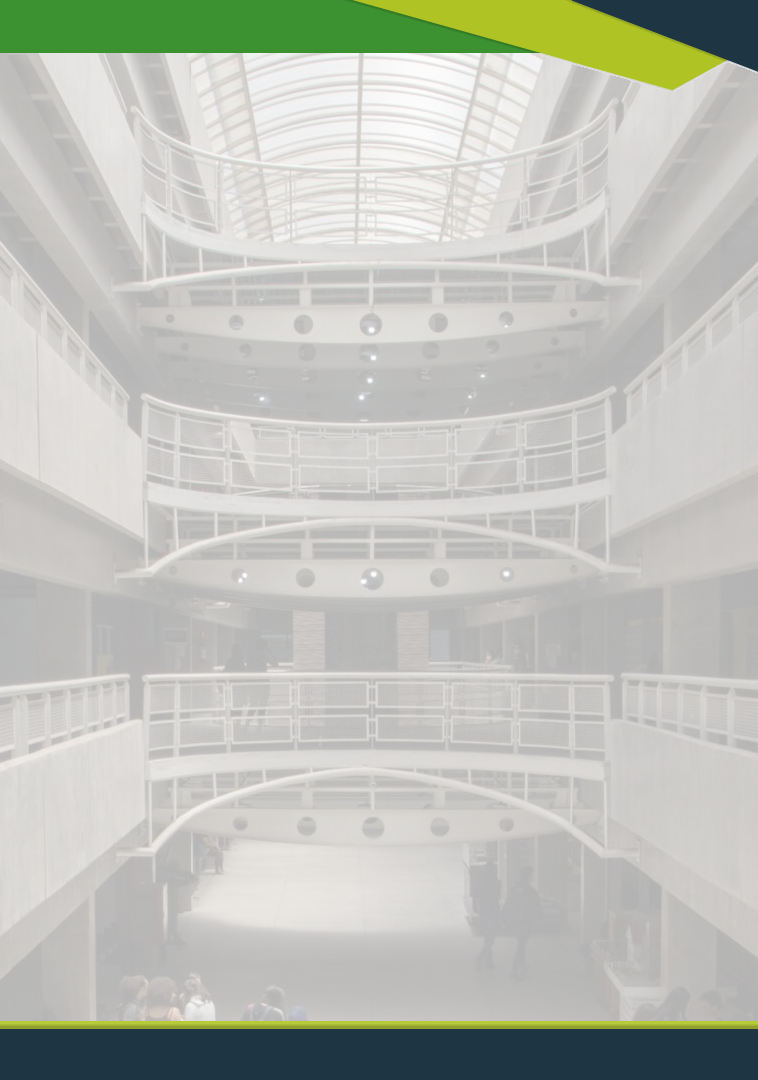
\includegraphics[width=\paperwidth]{Pictures/background.png}};
\draw (current page.center) node [fill=ocre,text opacity=1,inner sep=1cm]{\color{chapterhead}\Huge\centering\bfseries\sffamily\parbox[c][][t]{\paperwidth}{\centering \namesubject\\[15pt] % Nome da Matéria
{\Large \namecycle}%%Período do ciclo
}};

\end{tikzpicture}

\vfill
\Large\centering\text\sffamily{\centering\color{ocre}\nameauthor}

\Large\centering\text\sffamily{\centering\color{ocre}{\namecourse}}%curso

\Large\centering\bfseries\sffamily{\centering\color{ocre}{\nameinstitute}}%Instituição

\endgroup





%---------------------------------------------------------------------
%	Página de Apresentação 
%---------------------------------------------------------------------

% Entrar no arquivo "aparesentacao.tex" e redigir o texto de apresentação da disciplina

\cleardoublepage
\newpage
~\vfill
\thispagestyle{empty}
\doublespacing 
%\noindent \textsc{Curso Superior em Gestão da Tecnologia da Informação - Instituto Federal Baiano, Campus Bom Jesus da Lapa}\\

\noindent 
Caro estudante,

Bem-vindos ao Ciclo (19 a 30 de abril) da disciplina de Banco de Dados I que tratará os conceitos teóricos para aprofundar seus conhecimentos sobre Banco de Dados no curso Superior em Gestão da Tecnologia da Informação do Instituto Federal Baiano – Campus Bom Jesus da Lapa.

Para que seu estudo se torne proveitoso e prazeroso, este ciclo foi organizada em 2 semanas, com temas e subtemas que, por sua vez, são subdivididos em seções (tópicos), atendendo aos objetivos do processo de ensino-aprendizagem.

Nesta primeira semana, trataremos sobre os conceitos de modelos de dados, procuraremos compreender os conceitos gerais sobre modelagem de dados (modelo de dados, Entidade-Relacionamento, Relacionamentos, Atributos Chaves, Normalização e Padronização).  

%No capítulo 2, descreveremos [...]. No capítulo 3, detalharemos [...]. Finalmente, no capítulo 4 refletiremos um pouco sobre [...].

Esperamos que, até o final deste ciclo vocês possam:

- Ampliar a compreensão sobre Banco de Dados;
- Conceituar os Sistemas Gerenciadores de Banco de Dados (SGDB);
- Compreender a importância da normalização de padronização;

Para tanto, teremos vídeo aulas expositivas que serão disponibilizadas em nosso Ambiente Virtual de Aprendizagem (AVA) do Instituto Federal Baiano, campus Bom Jesus da Lapa.

Porém, antes de iniciar a leitura, gostaríamos que vocês parassem um instante para refletir sobre algumas questões: Qual é a importância de Banco de Dados para as organizações?

Não se preocupe.  Não queremos que vocês respondam de imediato essa questão.  Mas esperamos que, até o final, vocês tenham respostas e também formulem outras perguntas.

Vamos, então, iniciar nossas aulas? Bons estudos!


\vspace{3cm}
\DTMlangsetup{showdayofmonth=false}
\noindent \textit{1ª Ed., \today }
\DTMlangsetup{showdayofmonth=true}

%---------------------------------------------------------------------
%	SUMÁRIO
%---------------------------------------------------------------------

% Não é necessário fazer modificação

\chapterimage{capitulo.png}
\pagestyle{empty}
\tableofcontents
\cleardoublepage
\pagestyle{fancy}

%-------------------------------------------------------------
%	INSTRUÇÕES
%-------------------------------------------------------------
%
% A partir deste ponto serão inseridos os capítulos da apostila através dos seguintes passos:
% 
% 1) Incluir um mini resumo de uma parte do documento com o comando "\parte{Nome da Parte}". (Opcional)
% 2) Adicionar uma nova pasta 
% 2) Incluir um capítulo com o comando "\input{"Caminho do Capítulo"}. Ex.: Caso queira incluir o capítulo 1 inserir o comando "\input{Capitulo 1/capitulo}".
% 
%-------------------------------------------------------------
%	DIVISÃO POR PARTES
%-------------------------------------------------------------

%\parte{Parte Um}  % Comente essa linha (ctrl+/) se não quiser dividir a apostila em partes
% Título do capítulo
\capitulo{A Natureza da Eletricidade} 
\label{cap1}

\mais{

\begin{center}
    \Large \textbf{Objetivo}
\end{center}

Ao final deste capítulo, espera-se que o estudante seja capaz de:

\begin{itemize}
    \item Compreender o que é eletricidade e suas formas de manifestação.
    \item Identificar diferentes formas de conversão de energia envolvendo eletricidade.
    \item Distinguir os tipos de eletricidade: eletrostática, eletrodinâmica e eletromagnetismo.
    \item Reconhecer a estrutura básica do átomo e a relação entre elétrons e condução elétrica.
    \item Classificar materiais como condutores ou isolantes com base em suas propriedades elétricas.
    \item Aplicar corretamente os conceitos de corrente, tensão, resistência e potência elétrica.
    \item Explicar os princípios de atração e repulsão entre cargas elétricas.
    \item Entender os processos de eletrização por atrito, contato e indução.
    \item Relacionar fenômenos do cotidiano com os princípios da eletrostática.
\end{itemize}
}

\section{Introdução}

A eletricidade é um fenômeno físico fundamental, presente em praticamente todos os aspectos da vida moderna. Ela pode ser compreendida como uma forma de energia, cuja produção e conversão podem ocorrer de diversas maneiras. Neste capítulo, exploraremos os conceitos básicos sobre a natureza da eletricidade, as formas de geração e conversão de energia, os tipos de eletricidade e os princípios físicos que regem seu comportamento.

\section{Formas de Conversão de Energia}

A eletricidade pode ser gerada a partir de diferentes fontes de energia. Algumas das principais conversões de energia incluem:

\begin{itemize}
    \item \textbf{Energia química para elétrica:} como ocorre em pilhas e baterias.
    \item \textbf{Energia elétrica para energia química:} como no processo de eletrólise.
    \item \textbf{Energia térmica para elétrica:} usada, por exemplo, em baterias termonucleares de sondas espaciais.
    \item \textbf{Energia elétrica para térmica:} como ocorre em ferros de passar roupa e sanduicheiras.
    \item \textbf{Energia luminosa para elétrica:} como nas células fotovoltaicas.
    \item \textbf{Energia elétrica para luminosa:} como nas lâmpadas em geral.
    \item \textbf{Energia mecânica para elétrica:} como nos geradores.
    \item \textbf{Energia elétrica para mecânica:} como nos motores elétricos.
\end{itemize}

A eficiência das conversões pode variar conforme o tipo de energia de origem e de destino, sendo necessário, muitas vezes, passar por múltiplas etapas até alcançar uma forma de energia útil de maneira eficiente.

\subsection*{Exemplo: Lanterna Elétrica}

Um exemplo didático para ilustrar a conversão de energia é o funcionamento de uma lanterna simples:

\begin{itemize}
    \item \textbf{Fonte de energia:} pilhas conectadas em série (ex.: 3 pilhas de 1,5 V = 4,5 V).
    \item \textbf{Condutores:} partes metálicas internas que permitem a passagem dos elétrons.
    \item \textbf{Chave liga/desliga:} controla o fluxo de corrente elétrica.
    \item \textbf{Lâmpada:} transforma energia elétrica em energia luminosa e térmica.
\end{itemize}

Ao ligar a lanterna, a energia química das pilhas é convertida em energia elétrica, que percorre os condutores, acionando a lâmpada e convertendo-se em luz e calor.

\section{Tipos de Eletricidade}

A eletricidade pode ser dividida, de maneira geral, em três categorias principais:

\begin{itemize}
    \item \textbf{Eletrostática:} estuda as cargas elétricas em repouso.
    \item \textbf{Eletrodinâmica:} estuda as cargas elétricas em movimento.
    \item \textbf{Eletromagnetismo:} estuda a interação entre eletricidade e magnetismo.
\end{itemize}

A eletrodinâmica é a mais utilizada no nosso cotidiano, enquanto a eletrostática está presente em fenômenos como o choque ao encostar em uma maçaneta ou os raios durante tempestades.

\section{Estrutura do Átomo}

Compreender a eletricidade requer uma noção básica da estrutura do átomo:

\begin{itemize}
    \item \textbf{Núcleo:} formado por prótons (carga positiva) e nêutrons (sem carga).
    \item \textbf{Eletrosfera:} região ao redor do núcleo onde se localizam os elétrons (carga negativa).
\end{itemize}

Os elétrons mais externos do átomo são mais facilmente removíveis e, portanto, os principais responsáveis pela condução elétrica nos materiais.

\section{Condutores e Isolantes}
Os materiais se classificam quanto à sua capacidade de conduzir corrente elétrica:

\begin{itemize}
    \item \textbf{Condutores:} permitem o livre movimento dos elétrons. Exemplos: metais como cobre, prata, alumínio, ferro, chumbo, ouro, além de ligas como bronze e constantan. Alguns líquidos, como soluções salinas, também conduzem eletricidade.
    
    \item \textbf{Isolantes:} dificultam o movimento dos elétrons. Exemplos: madeira seca, vidro, borracha, plásticos. Contudo, não existe isolante perfeito — todo material tem um limite de tensão, acima do qual pode se tornar condutor.
\end{itemize}

O ar, por exemplo, normalmente é isolante, mas pode se tornar condutor quando submetido a uma tensão suficientemente alta, como no caso dos raios.

\section{Conceitos Fundamentais}
Antes de avançarmos, é importante revisar alguns conceitos essenciais:

\begin{itemize}
    \item \textbf{Tensão elétrica (ou diferença de potencial):} é a "força" que impulsiona os elétrons em um circuito. Sua unidade é o Volt (V).
    
    \item \textbf{Corrente elétrica:} é o movimento ordenado dos elétrons em um condutor. Sua unidade é o Ampère (A).
    
    \item \textbf{Resistência elétrica:} é a oposição à passagem da corrente elétrica. Sua unidade é o Ohm (\Omega).
    
    \item \textbf{Potência elétrica:} é a quantidade de energia consumida ou gerada por unidade de tempo. Sua unidade é o Watt (W).
\end{itemize}

\section{Princípios de Atração e Repulsão}
Um dos primeiros fenômenos observados na história da eletricidade foi o de atração e repulsão entre cargas elétricas, descrito pela \textbf{Lei de Du Fay}:

\begin{itemize}
    \item Cargas de mesmo sinal se repelem.
    \item Cargas de sinais opostos se atraem.
\end{itemize}

\section{Princípio da Conservação das Cargas Elétricas}
A \textbf{conservação da carga elétrica} afirma que as cargas elétricas não podem ser criadas nem destruídas, apenas transferidas. Em um sistema isolado, a soma algébrica das cargas antes e depois de um processo de eletrização permanece constante.

\section{Processos de Eletrização}
Os corpos podem adquirir carga elétrica por três métodos principais:

\subsection*{a) Eletrização por Atrito}
Neste processo, dois materiais inicialmente neutros são atritados. O atrito provoca a transferência de elétrons de um corpo para outro, fazendo com que um fique eletricamente negativo (com excesso de elétrons) e o outro positivo (com falta de elétrons).

\textit{Exemplo:} atritar um pente em um pedaço de tecido e depois aproximá-lo de pedacinhos de papel.

\subsection*{b) Eletrização por Contato}
Um corpo previamente eletrizado encosta em outro corpo condutor neutro. Como resultado, há uma redistribuição de cargas, e o corpo neutro passa a apresentar carga elétrica semelhante à do corpo eletrizado.

\subsection*{c) Eletrização por Indução}
Neste processo, um corpo eletrizado é aproximado de um corpo neutro, sem que haja contato físico. O campo elétrico do corpo eletrizado provoca uma separação de cargas no corpo neutro (polarização). A seguir, ao se conectar esse corpo neutro à terra, parte das cargas será escoada, e ao desconectá-lo da terra, ele ficará eletrizado com carga oposta à do indutor.

\subsection{Exemplos Práticos de Eletrização}
Diversos experimentos simples podem demonstrar os fenômenos da eletrização. Alguns exemplos:

\begin{itemize}
    \item \textbf{Eletrização por atrito com balões:} ao esfregar um balão em cabelos secos ou em tecido de lã, o balão pode atrair pedaços de papel ou até grudar temporariamente em uma parede.
    
    \item \textbf{Canudos plásticos:} ao atritar canudos plásticos com pano e aproximá-los de pequenos corpos leves ou outros canudos, observamos repulsão ou atração, dependendo da carga acumulada.
    
    \item \textbf{Disco de pizza e bolinhas metálicas:} usando discos plásticos, pano e bolinhas metálicas suspensas por fios, pode-se montar um experimento para observar o armazenamento e a transferência de eletricidade estática.
\end{itemize}

Vídeos demonstrativos desses experimentos serão disponibilizados no material complementar da disciplina.

\subsection{Aplicações e Ocorrências da Eletricidade Estática}
A eletricidade estática está presente em diversas situações cotidianas:

\begin{itemize}
    \item \textbf{Descargas eletrostáticas:} ao caminhar sobre certos pisos com sapatos isolantes e encostar em objetos metálicos, pode-se sentir um leve choque.
    \item \textbf{Clima e atmosfera:} os raios são exemplos de descarga eletrostática entre nuvens ou entre nuvens e o solo.
    \item \textbf{Indústria:} controle de eletricidade estática é fundamental em ambientes industriais, especialmente com componentes eletrônicos sensíveis.
\end{itemize}

\section{Recapitulando}
Neste capítulo, aprendemos que:

\begin{itemize}
    \item A eletricidade é uma forma de energia resultante do movimento ou acúmulo de cargas elétricas.
    \item Ela pode ser gerada e convertida por diferentes formas de energia.
    \item Existem três formas de eletrização: atrito, contato e indução.
    \item Conhecimentos básicos sobre átomos, materiais condutores e isolantes são essenciais para o entendimento da eletricidade.
    \item A eletricidade estática está presente em fenômenos naturais e experimentos simples do cotidiano.
\end{itemize}

\section{Atividades Sugeridas}
\begin{enumerate}
    \item Explique com suas palavras a diferença entre eletrostática e eletrodinâmica.
    \item Liste 3 exemplos de conversão de energia que envolvem eletricidade.
    \item Faça um experimento caseiro de eletrização por atrito usando balões, canudos ou pentes, e registre suas observações.
    \item Desenhe o modelo atômico e indique onde se localizam os prótons, nêutrons e elétrons.
\end{enumerate}

\section{Material Complementar}

\midia{ O vídeo produzido pela TV Unifesp, apresenta demonstrações práticas dos processos de eletrização, e está disponível no link
\url{https://www.youtube.com/watch?v=MvV46hVy3_Y}.}

\vspace{1cm}
\noindent\textbf{Próximo capítulo:} \hyperref[cap2]{Lei de Ohm e Corrente Elétrica.}
 % Adiciona  capítulo na parte 1. Para escrever o capítulo 1, abra o arquivo "/Capitulo 1/capitulo1.tex". O mesmo raciocínio vale para os demais.
% Título do capítulo
\capitulo{Lei de Ohm e Corrente Elétrica}\label{cap2}

\mais{

\begin{center}
    \Large \textbf{Objetivo}
\end{center}

Ao final deste capítulo, espera-se que o estudante seja capaz de:

\begin{itemize}
    \item Compreender o conceito de corrente elétrica e sua definição matemática.
    \item Diferenciar corrente real e corrente convencional.
    \item Reconhecer os diversos tipos de materiais condutores: metálicos, líquidos e gasosos.
    \item Utilizar corretamente a Primeira Lei de Ohm para relacionar tensão, corrente e resistência.
    \item Aplicar a Segunda Lei de Ohm para calcular a resistência em função das propriedades do condutor.
    \item Interpretar tabelas de resistividade e compreender a influência da temperatura na resistência elétrica.
    \item Efetuar cálculos com múltiplos e submúltiplos das unidades elétricas.
    \item Resolver problemas práticos envolvendo a Lei de Ohm em diferentes contextos.
\end{itemize}
}

\secao{Introdução}
\index{seção}

Neste capítulo, abordaremos a Lei de Ohm, uma das mais importantes leis da eletricidade, que estabelece a relação entre tensão elétrica, corrente e resistência. Vamos também relembrar conceitos fundamentais da eletrodinâmica, explorar os tipos de corrente e discutir os materiais condutores.

\section{Eletrodinâmica: O Início}

A eletrodinâmica teve grande avanço com a invenção da pilha elétrica por Alessandro Volta. Antes disso, os estudos em eletricidade limitavam-se a fenômenos eletrostáticos, como a eletrização por atrito.

A pilha de Volta consistia em discos alternados de cobre e zinco, separados por feltros embebidos em solução ácida. Essa configuração permitia gerar uma diferença de potencial entre os terminais.

\section{Geradores de Corrente}

Os geradores podem ser classificados em:

\begin{itemize}
    \item \textbf{Geradores de corrente contínua (CC):} como pilhas e baterias.
    \item \textbf{Geradores de corrente alternada (CA):} usados em usinas hidroelétricas, termelétricas, entre outras.
\end{itemize}

\section{Sentido da Corrente Elétrica}

A corrente elétrica é o movimento ordenado dos elétrons através de um condutor. Esse movimento real ocorre do polo negativo para o polo positivo do gerador. No entanto, por convenção, a corrente elétrica é representada como fluindo do polo positivo para o negativo, chamada de \textbf{corrente convencional}.

Ambos os sentidos não ocorrem simultaneamente. A corrente real representa o fluxo físico de elétrons; a convencional é adotada por convenção para facilitar a análise de circuitos.

\section{Materiais Condutores de Eletricidade}

Existem diferentes tipos de materiais capazes de conduzir corrente elétrica:

\begin{itemize}
    \item \textbf{Condutores metálicos:} metais como cobre, alumínio, ouro, prata e ferro, com presença de elétrons livres.
    \item \textbf{Condutores líquidos:} soluções eletrolíticas, como água com sais ou ácidos, que possuem íons livres.
    \item \textbf{Condutores gasosos:} requerem alta diferença de potencial para se ionizarem e permitirem a passagem de corrente.
\end{itemize}

\section{Definição de Corrente Elétrica}

A corrente elétrica ($I$) é definida como a quantidade de carga ($Q$), em coulombs, que passa por uma seção transversal de um condutor em um intervalo de tempo ($\Delta t$):

\[
I = \frac{Q}{\Delta t}
\]

A unidade de medida da corrente elétrica é o \textbf{ampère (A)}. Um ampère equivale a um coulomb por segundo:

\[
1\,\text{A} = 1\,\text{C/s}
\]

\section{Medição de Corrente e Tensão Elétrica}

Para medir corrente elétrica, utilizamos um \textbf{amperímetro}, que deve ser conectado em \textbf{série} com a carga no circuito.

Para medir tensão elétrica (diferença de potencial), usamos um \textbf{voltímetro}, que deve ser conectado em \textbf{paralelo} com o componente.

Hoje em dia, o \textbf{multímetro} é um instrumento muito utilizado para medir várias grandezas, como corrente, tensão e resistência.


\section{Resistência Elétrica}

A resistência elétrica ($R$) representa a oposição que um material oferece à passagem da corrente elétrica. Depende do tipo de material, do comprimento e da área da seção transversal do condutor.

A unidade de medida da resistência é o \textbf{ohm ($\Omega$)}:

\[
1\,\Omega = \frac{1\,\text{V}}{1\,\text{A}}
\]

\section{Primeira Lei de Ohm}

Formulada por Georg Simon Ohm, esta lei estabelece que, em um condutor ôhmico, a corrente elétrica ($I$) é diretamente proporcional à tensão elétrica ($V$) e inversamente proporcional à resistência ($R$):

\[
I = \frac{V}{R}
\]

As formas alternativas da equação são:

\[
V = R \cdot I \quad \text{ou} \quad R = \frac{V}{I}
\]

\textbf{Triângulo REI:} Um método mnemônico útil para lembrar as fórmulas:

\[
\begin{array}{c}
\boxed{V} \\
\boxed{R \quad I}
\end{array}
\]

\section{Segunda Lei de Ohm}

A Segunda Lei de Ohm descreve como a resistência elétrica de um fio depende de suas propriedades físicas:

\[
R = \rho \cdot \frac{L}{A}
\]

Onde:

\begin{itemize}
    \item $R$: resistência elétrica (\(\Omega\))
    \item $\rho$: resistividade do material (\(\Omega \cdot \text{m}\) ou \(\Omega \cdot \text{mm}^2/\text{m}\))
    \item $L$: comprimento do condutor (m)
    \item $A$: área da seção transversal (\(\text{mm}^2\) ou \(\text{mm}^2)\))
\end{itemize}

\subsection{Tabela de Resistividade de Materiais}

\begin{center}
\begin{tabular}{|l|c|}
\hline
\textbf{Material} & \textbf{Resistividade (\(\Omega \cdot \text{mm}^2/\text{m}\)) a 20$^{\circ}$C} \\
\hline
Prata & \(1,59 \times 10^{-2}\) \\
Cobre & \(1,68 \times 10^{-2}\) \\
Ouro & \(2,44 \times 10^{-2}\) \\
Alumínio & \(2,82 \times 10^{-2}\) \\
Constantan (liga) & \(49 \times 10^{-2}\) \\
Níquel & \(6,99 \times 10^{-2}\) \\
\hline
\end{tabular}
\end{center}

\textbf{Observações:}
\begin{itemize}
    \item Materiais com menor resistividade conduzem melhor.
    \item Materiais como o ouro, embora mais caros, são usados em contatos elétricos por sua resistência à oxidação.
    \item Ligas como \textit{Constantan} são preferidas na fabricação de resistores devido à baixa variação com a temperatura.
\end{itemize}

\subsection{Influência da Temperatura}

A resistividade varia com a temperatura. Em metais condutores, a resistividade aumenta com a elevação da temperatura. Já em ligas específicas (como Constantan), essa variação é muito menor, o que as torna ideais para componentes eletrônicos.

\section{Exercícios Resolvidos}

\subsection*{Exemplo 1: O Pássaro no Fio}
Um pássaro pousa em um fio de alta tensão que conduz uma corrente de $1000\,\text{A}$. A resistência por metro do fio é $5 \times 10^{-5}\,\Omega/\text{m}$ e a distância entre os pés do pássaro é de $6\,\text{cm}$. Qual a diferença de potencial entre os pés do pássaro?

\textbf{Resolução:}
\begin{itemize}
    \item Convertendo $6\,\text{cm} = 0{,}06\,\text{m}$
    \item Resistência correspondente:
    \[
    R = \left(5 \times 10^{-5}\right) \times 0{,}06 = 3 \times 10^{-6}\,\Omega
    \]
    \item Tensão elétrica:
    \[
    V = R \cdot I = \left(3 \times 10^{-6}\right) \cdot 1000 = 3 \times 10^{-3}\,\text{V} = 3\,\text{mV}
    \]
\end{itemize}

\textbf{Conclusão:} A diferença de potencial é muito pequena para causar dano ao pássaro: apenas $3\,\text{mV}$.

\subsection*{Exemplo 2: Resistência de um Cabo}
Um cabo de transmissão é formado por 7 fios de cobre, cada um com $10\,\text{mm}^2$ de área. Qual a resistência elétrica para um comprimento de $1\,\text{km}$, dado que $\rho = 2{,}1 \times 10^{-2}\,\Omega \cdot \text{mm}^2/\text{m}$?

\textbf{Resolução:}
\begin{itemize}
    \item Área total: $A = 7 \times 10 = 70\,\text{mm}^2$
    \item Comprimento: $L = 1000\,\text{m}$
    \item Aplicando a segunda lei de Ohm:
    \[
    R = \rho \cdot \frac{L}{A} = 2{,}1 \times 10^{-2} \cdot \frac{1000}{70} = 0{,}3\,\Omega
    \]
\end{itemize}

\subsection*{Exemplo 3: Tensão Elétrica}
Um resistor de $100\,\Omega$ é percorrido por uma corrente de $2{,}5\,\text{A}$. Qual a tensão?

\[
V = R \cdot I = 100 \cdot 2{,}5 = 250\,\text{V}
\]

\subsection*{Exemplo 4: Resistência}
Um resistor é ligado a $110\,\text{V}$ e conduz uma corrente de $5\,\text{A}$. Qual sua resistência?

\[
R = \frac{V}{I} = \frac{110}{5} = 22\,\Omega
\]

\subsection*{Exemplo 5: Corrente Elétrica}
Um resistor de $200\,\Omega$ está ligado a uma fonte de $300\,\text{V}$. Qual a corrente?

\[
I = \frac{V}{R} = \frac{300}{200} = 1{,}5\,\text{A}
\]

\subsection*{Exemplo 6: Corrente em Circuito Automotivo}
Um resistor de $6\,\Omega$ é ligado a uma bateria de $12\,\text{V}$. Qual a corrente elétrica?

\[
I = \frac{12}{6} = 2\,\text{A}
\]

\section{Notação Científica e Unidades}

\begin{itemize}
    \item \textbf{Múltiplos:} 
        \begin{itemize}
            \item $1\,\text{k} = 10^3 = 1000$
            \item $1\,\text{M} = 10^6 = 1\,000\,000$
        \end{itemize}
    \item \textbf{Submúltiplos:}
        \begin{itemize}
            \item $1\,\text{m} = 10^{-3}$
            \item $1\,\mu = 10^{-6}$
        \end{itemize}
    \item \textbf{Representação correta:} número + espaço + unidade (ex.: $2{,}5\,\text{A}$).
    \item \textbf{Separador decimal:} utilizar vírgula (ex.: $3{,}14$), e não ponto.
    \item \textbf{Números grandes:} não utilizar ponto entre milhares (ex.: $10000$, e não $10.000$).
\end{itemize}

O material extra sobre notação científica e unidades serão disponibilizados no material complementar.

\section{Considerações Finais}

Neste capítulo, abordamos a corrente elétrica, os tipos de condutores, a resistência e as leis fundamentais de Ohm. Compreender esses conceitos é essencial para o estudo de circuitos elétricos e aplicações em eletrônica, instalações e equipamentos.

\section{Material Complementar}

\midia{O site do INMETRO possui um documento sobre o Sistema Internacional de Medidas, e em especial ao \textbf{capítulo 3} (Múltiplos e submúltiplos decimais das unidades do SI), \textbf{seção 5.4.2} (Símbolos das grandezas e das unidades), \textbf{seção 5.4.3} (Escrita do valor de uma grandeza) e \textbf{seção 5.4.4} (Escrita dos números e separador decimal), são importantes para a disciplina. O material está disponível no link
\url{https://www.gov.br/inmetro/pt-br/centrais-de-conteudo/publicacoes/documentos-tecnicos-em-metrologia/si_versao_final.pdf}.}

\noindent\textbf{Próximo capítulo:} \hyperref[cap3]{Associação de Resistores.}



%\parte{Parte Dois}  % Comente essa linha (ctrl+/) se não quiser dividir a apostila em partes
% Título do capítulo
\capitulo{Associação de Resistores}\label{cap3}

\mais{

\begin{center}
    \Large \textbf{Objetivo}
\end{center}

Ao final deste capítulo, espera-se que o estudante seja capaz de:

\begin{itemize}
    \item Compreender os conceitos de associação em série e paralelo de resistores.
    \item Calcular a resistência equivalente em associações simples.
    \item Reconhecer as características elétricas (tensão e corrente) nas diferentes associações.
    \item Identificar situações reais onde resistores são associados em série ou paralelo.
    \item Resolver circuitos com associação mista de resistores, utilizando estratégias passo a passo.
    \item Avaliar os efeitos da resistência dos condutores nas quedas de tensão em circuitos reais.
    \item Aplicar os conhecimentos em contextos práticos, como instalações elétricas residenciais e automotivas.
    \item Verificar se os resultados obtidos em cálculos são coerentes com os princípios teóricos.
\end{itemize}
}

\section{Revisão: Leis de Ohm}
Antes de iniciarmos o estudo sobre associações de resistores, vamos relembrar brevemente as duas Leis de Ohm.

\subsection*{Primeira Lei de Ohm}
A corrente elétrica ($I$) que percorre um condutor é diretamente proporcional à tensão ($V$) aplicada e inversamente proporcional à resistência elétrica ($R$):

\[
I = \frac{V}{R}
\quad \text{ou} \quad V = R \cdot I \quad \text{ou} \quad R = \frac{V}{I}
\]

\textbf{Triângulo REI}:

\[
\begin{array}{c}
\boxed{V} \\
\boxed{R \quad I}
\end{array}
\]

\subsection*{Segunda Lei de Ohm}
A resistência elétrica de um condutor é dada por:

\[
R = \rho \cdot \frac{L}{A}
\]

Onde:
\begin{itemize}
    \item $R$: resistência do fio (\(\Omega\))
    \item $\rho$: resistividade do material
    \item $L$: comprimento do condutor (m)
    \item $A$: área da seção transversal (m²)
\end{itemize}

\section{Associação de Resistores}
\index{seção}

\subsection{Associação de Resistores em Série}
A associação em série ocorre quando os resistores estão ligados um após o outro, em sequência, de modo que a mesma corrente percorre todos os componentes.

%\begin{center}
%\includegraphics[width=0.6\textwidth]{serie.png} % imagem a ser adicionada futuramente
%\end{center}

\subsubsection{Características:}
\begin{itemize}
    \item \textbf{A corrente ($I$) é a mesma em todos os resistores}.
    \item \textbf{A tensão total} é a soma das quedas de tensão individuais:
    \[
    V = V_1 + V_2 + V_3 + \dots + V_n
    \]
    \item Cada queda de tensão ($V_i$) pode ser obtida pela Lei de Ohm:
    \[
    V_i = R_i \cdot I
    \]
\end{itemize}

\subsubsection{Resistência Equivalente em Série}
A resistência total é a soma das resistências:

\[
R_{eq} = R_1 + R_2 + R_3 + \dots + R_n
\]

\subsubsection{Aplicação Prática}
Considere três lâmpadas incandescentes idênticas ligadas em série em uma tomada de $110\,\text{V}$. Cada lâmpada receberá apenas $\frac{1}{3}$ da tensão, resultando em menor luminosidade. Se uma lâmpada queimar, o circuito será interrompido — todas as demais também apagarão.

\subsubsection{Exemplo Resolvido: Queda de Tensão em Condutores}
Uma bateria de $24\,\text{V}$ alimenta uma carga de $3\,\Omega$ através de dois fios, cada um com resistência de $0{,}5\,\Omega$. Determine a tensão na carga.

\textbf{Solução:}
\begin{itemize}
    \item Resistência equivalente: $0{,}5 + 3 + 0{,}5 = 4\,\Omega$
    \item Corrente total:
    \[
    I = \frac{V}{R} = \frac{24}{4} = 6\,\text{A}
    \]
    \item Tensão sobre a carga:
    \[
    V_{\text{carga}} = R_{\text{carga}} \cdot I = 3 \cdot 6 = 18\,\text{V}
    \]
\end{itemize}

\textbf{Conclusão:} Mesmo com uma fonte de $24\,\text{V}$, a carga recebe apenas $18\,\text{V}$ devido às perdas nos condutores.

\subsection{Associação de Resistores em Paralelo}
Na associação em paralelo, os resistores estão ligados de modo que seus terminais estejam conectados aos mesmos pontos. Isso significa que a tensão sobre cada resistor é a mesma.

%\begin{center}
%\includegraphics[width=0.6\textwidth]{paralelo.png} % imagem a ser adicionada futuramente
%\end{center}

\subsubsection{Características:}
\begin{itemize}
    \item \textbf{A tensão ($V$) é igual para todos os resistores}:
    \[
    V = V_1 = V_2 = V_3 = \dots = V_n
    \]
    \item \textbf{A corrente total ($I$)} é dividida entre os resistores:
    \[
    I = I_1 + I_2 + I_3 + \dots + I_n
    \]
    \item Cada corrente individual pode ser calculada pela Lei de Ohm:
    \[
    I_i = \frac{V}{R_i}
    \]
\end{itemize}

\subsubsection{Resistência Equivalente em Paralelo}
A fórmula geral para a resistência equivalente é:

\[
\frac{1}{R_{eq}} = \frac{1}{R_1} + \frac{1}{R_2} + \frac{1}{R_3} + \dots + \frac{1}{R_n}
\]

\textbf{Fórmula genérica:}
\[
\frac{1}{R_{eq}} = \sum_{i=1}^{n} \frac{1}{R_i}
\]

\subsubsection{Casos Especiais}
\begin{itemize}
    \item \textbf{Resistores com o mesmo valor:}
    \[
    R_{eq} = \frac{R}{n}
    \]
    Onde $R$ é o valor de cada resistor e $n$ é a quantidade de resistores.

    \item \textbf{Dois resistores apenas:} produto pela soma:
    \[
    R_{eq} = \frac{R_1 \cdot R_2}{R_1 + R_2}
    \]
\end{itemize}

\subsubsection{Importante:}
O valor da resistência equivalente de uma associação em paralelo \textbf{sempre será menor} que o menor resistor da associação.

\textbf{Exemplo:}
Para resistores de $10\,\Omega$, $20\,\Omega$ e $5\,\Omega$ em paralelo, o valor de $R_{eq}$ será menor que $5\,\Omega$.

\subsubsection{Aplicação: Instalações Elétricas}
Em circuitos elétricos residenciais, os dispositivos (lâmpadas, tomadas, etc.) são ligados em paralelo, para que todos recebam a mesma tensão da rede (geralmente $127\,\text{V}$ ou $220\,\text{V}$). A corrente é dividida conforme a resistência de cada aparelho.

\subsection{Observações Práticas}
\subsubsection{Queda de Tensão em Condutores}
Condutores reais apresentam resistência, mesmo que pequena. Em casos de alta corrente ou grandes comprimentos, essa resistência pode causar quedas de tensão significativas.

\textbf{Exemplo prático:} Instalações de chuveiros elétricos.

\begin{itemize}
    \item Um chuveiro elétrico pode demandar de $25$ a $35\,\text{A}$ de corrente.
    \item Se os condutores forem finos (com seção transversal pequena), a resistência será maior.
    \item Isso pode provocar aquecimento dos cabos, queda de desempenho e até risco de incêndio.
    \item Por isso, utilizam-se cabos de \textbf{4 mm²} ou \textbf{6 mm²} para chuveiros.
\end{itemize}

\subsubsection{Instalações Automotivas}
Em automóveis, problemas de queda de tensão podem ocorrer devido à má conexão entre a bateria e o chassi. Esse tipo de problema é comum quando a \textbf{cordoalha de aterramento} está com mau contato, resultando em dificuldades de partida, falhas de recarga da bateria ou funcionamento irregular de componentes eletrônicos.

\subsection{Comparativo: Série vs. Paralelo}

\begin{center}
\begin{tabular}{|l|c|c|}
\hline
\textbf{Característica} & \textbf{Série} & \textbf{Paralelo} \\
\hline
Tensão & Dividida & Igual em todos os resistores \\
Corrente & Igual em todos os resistores & Dividida \\
Fórmula de $R_{eq}$ & Soma direta & Soma dos inversos \\
Comportamento se um resistor queimar & Abre todo o circuito & Os demais continuam funcionando \\
\hline
\end{tabular}
\end{center}

\section{Considerações Finais}
Neste capítulo, você aprendeu:

\begin{itemize}
    \item Como funcionam as associações em série e paralelo.
    \item Como aplicar a Lei de Ohm para calcular tensões, correntes e resistências equivalentes.
    \item Como essas associações se aplicam em instalações elétricas residenciais e automotivas.
    \item Que o correto dimensionamento de cabos influencia diretamente no funcionamento e segurança dos circuitos.
\end{itemize}

\textbf{Dica:} sempre verifique se o valor da resistência equivalente faz sentido. Em série, deve ser maior que qualquer uma das individuais. Em paralelo, deve ser menor que a menor delas.

\vspace{0.5cm}
\noindent\textbf{Próximo capítulo:} \hyperref[cap4]{Exercícios sobre Associação de Resistores.} % Adicionar  capítulo na parte 2
% Título do capítulo
\capitulo{Exercícios sobre Associação de Resistores}\label{cap4}

\mais{

\begin{center}
    \Large \textbf{Objetivo}
\end{center}

Ao final deste capítulo, espera-se que o estudante seja capaz de:

\begin{itemize}
    \item Resolver exercícios aplicados sobre associação de resistores em série e paralelo.
    \item Aplicar corretamente fórmulas para cálculo da resistência equivalente.
    \item Realizar conversão entre unidades de resistência (ohm, quilohm, megaohm).
    \item Identificar visualmente associações em série, paralelo e mista, independentemente da orientação do desenho.
    \item Utilizar estratégias passo a passo para resolver associações mistas.
    \item Verificar a coerência dos resultados com base em princípios teóricos.
    \item Reforçar os conceitos estudados nos capítulos anteriores por meio da prática.
\end{itemize}
}

\secao{Exercícios sobre Associação de Resistores}
\index{seção}

\subsection{Revisão: Associação em Série}
Na associação em série, a \textbf{resistência equivalente} é a soma direta dos resistores ligados em sequência:

\[
R_{eq} = R_1 + R_2 + R_3 + \dots + R_n
\]

\textbf{Importante:} Todos os resistores devem estar na mesma unidade para que a soma seja válida.

\subsubsection{Exemplo 1}
Dois resistores de $100\,\Omega$ em série entre os pontos A e B:

\[
R_{eq} = 100 + 100 = 200\,\Omega
\]

\subsubsection{Exemplo 2}
Um resistor de $50\,\Omega$ e outro de $145\,\Omega$:

\[
R_{eq} = 50 + 145 = 195\,\Omega
\]

\subsubsection{Exemplo 3: Conversão de Unidades}
Um resistor de $1\,\text{k}\Omega$ e outro de $220\,\Omega$:

\[
1\,\text{k}\Omega = 1000\,\Omega
\quad \Rightarrow \quad
R_{eq} = 1000 + 220 = 1220\,\Omega
\]

\subsubsection{Exemplo 4}
$2{,}5\,\text{k}\Omega$ e $560\,\Omega$:

\[
2{,}5\,\text{k}\Omega = 2500\,\Omega
\quad \Rightarrow \quad
R_{eq} = 2500 + 560 = 3060\,\Omega
\]

\subsubsection{Exemplo 5}
Resistores: $100\,\text{k}\Omega$, $550\,\Omega$ e $6000\,\Omega$:

\[
100\,\text{k}\Omega = 100000\,\Omega
\quad \Rightarrow \quad
R_{eq} = 100000 + 550 + 6000 = 106550\,\Omega
\]

\subsubsection{Exemplo 6: Megaohms e kilohms}
Resistores: $1\,\text{M}\Omega$, $620\,\text{k}\Omega$, $1000\,\Omega$:

\[
1\,\text{M}\Omega = 1000000\,\Omega,\quad
620\,\text{k}\Omega = 620000\,\Omega
\quad \Rightarrow \quad
R_{eq} = 1000000 + 620000 + 1000 = 1621000\,\Omega
\]

\subsubsection{Nota:}
A ordem e disposição dos resistores (horizontal, vertical, zigue-zague) não altera a configuração elétrica. O importante é observar como os terminais estão conectados em sequência.

\subsubsection{Exemplo 7}
$72\,\text{k}\Omega$ + $330\,\text{k}\Omega$:

\[
R_{eq} = 72 + 330 = 402\,\text{k}\Omega
\]

Ou, em ohms:

\[
72000 + 330000 = 402000\,\Omega
\]

\subsubsection{Exemplo 8: Resistores em zigue-zague}
$30\,\text{k}\Omega$, $20\,\text{k}\Omega$, $10\,\text{k}\Omega$:

\[
R_{eq} = 30 + 20 + 10 = 60\,\text{k}\Omega = 60000\,\Omega
\]

\subsection{Revisão: Associação em Paralelo}
Na associação em paralelo, a \textbf{tensão elétrica é a mesma} em todos os resistores, e a \textbf{corrente se divide} de acordo com o valor da resistência.

A resistência equivalente é dada pela fórmula geral:

\[
\frac{1}{R_{eq}} = \frac{1}{R_1} + \frac{1}{R_2} + \dots + \frac{1}{R_n}
\]

\textbf{Importante:} O resultado da resistência equivalente será sempre \textbf{menor que o menor resistor da associação}.

\subsubsection{Casos Particulares}
\begin{itemize}
    \item \textbf{Resistores iguais:}
    \[
    R_{eq} = \frac{R}{n}
    \]

    \item \textbf{Dois resistores apenas:}
    \[
    R_{eq} = \frac{R_1 \cdot R_2}{R_1 + R_2}
    \]
\end{itemize}

\subsubsection{Exemplo 1: Dois resistores diferentes}
$R_1 = 100\,\Omega$, $R_2 = 50\,\Omega$

\[
\frac{1}{R_{eq}} = \frac{1}{100} + \frac{1}{50} = \frac{3}{100}
\Rightarrow
R_{eq} = \frac{100}{3} \approx 33{,}33\,\Omega
\]

\textit{Verificação:} $33{,}33\,\Omega < 50\,\Omega$ ✅

\subsubsection{Exemplo 2: Mesmo problema usando produto pela soma}
\[
R_{eq} = \frac{100 \cdot 50}{100 + 50} = \frac{5000}{150} = 33{,}33\,\Omega
\]

\subsubsection{Exemplo 3: Resistores de 25\,\Omega e 30\,\Omega}
\[
\frac{1}{R_{eq}} = \frac{1}{25} + \frac{1}{30}
= \frac{11}{150}
\Rightarrow R_{eq} \approx 13{,}63\,\Omega
\]

\textit{Verificação:} $13{,}63\,\Omega < 25\,\Omega$

\subsubsection{Exemplo 4: Três resistores distintos}
$R_1 = 30\,\Omega$, $R_2 = 60\,\Omega$, $R_3 = 90\,\Omega$

\[
\frac{1}{R_{eq}} = \frac{1}{30} + \frac{1}{60} + \frac{1}{90}
= \frac{6}{45} = \frac{2}{15}
\Rightarrow R_{eq} = \frac{15}{2} = 7{,}5\,\Omega
\]

\textit{Verificação:} $R_{eq} < 30\,\Omega$

\subsubsection{Exemplo 5: Três resistores iguais}
Três resistores de $30\,\Omega$:

\[
R_{eq} = \frac{30}{3} = 10\,\Omega
\]

Ou usando a fórmula geral:

\[
\frac{1}{R_{eq}} = \frac{1}{30} + \frac{1}{30} + \frac{1}{30}
= \frac{3}{30} = \frac{1}{10}
\Rightarrow R_{eq} = 10\,\Omega
\]

\subsubsection{Exemplo 6: Diversos valores}
$R_1 = 10\,\text{k}\Omega$, $R_2 = 300\,\Omega$, $R_3 = 1\,\text{k}\Omega$, $R_4 = 500\,\Omega$

\[
\frac{1}{R_{eq}} = \frac{1}{10000} + \frac{1}{300} + \frac{1}{1000} + \frac{1}{500}
\Rightarrow R_{eq} \approx 154{,}4\,\Omega
\]

\textit{Verificação:} $154{,}4\,\Omega < 300\,\Omega$ ✅

\subsection{Associação Mista de Resistores}
Associação mista ocorre quando resistores estão conectados em partes em série e outras em paralelo no mesmo circuito.

\subsubsection{Estratégia de Resolução}
\begin{enumerate}
    \item Identificar trechos que estão em paralelo e calcular sua resistência equivalente.
    \item Substituir os trechos calculados e verificar se restaram resistores em série.
    \item Repetir o processo até reduzir o circuito a uma única resistência equivalente entre os pontos A e B.
\end{enumerate}

\subsubsection{Exemplo 1: Paralelo seguido de série}
Resistores:
\[
\text{Paralelo: } R_1 = 100\,\Omega, R_2 = 200\,\Omega \quad\text{em paralelo}
\quad\text{em série com } R_3 = 300\,\Omega
\]

\begin{itemize}
    \item Primeiro, calcule o paralelo:
    \[
    \frac{1}{R_{12}} = \frac{1}{100} + \frac{1}{200} = \frac{3}{200} \Rightarrow R_{12} = \frac{200}{3} \approx 66{,}67\,\Omega
    \]
    \item Em seguida, calcule a série:
    \[
    R_{eq} = R_{12} + R_3 = 66{,}67 + 300 = 366{,}67\,\Omega
    \]
\end{itemize}

\subsubsection{Exemplo 2: Série seguida de paralelo}
Resistores:
\[
\text{Série: } R_1 = 300\,\Omega,\ R_2 = 400\,\Omega
\quad\text{em paralelo com } R_3 = 500\,\Omega
\]

\begin{itemize}
    \item Série:
    \[
    R_{12} = 300 + 400 = 700\,\Omega
    \]
    \item Paralelo com $R_3$:
    \[
    \frac{1}{R_{eq}} = \frac{1}{700} + \frac{1}{500} \Rightarrow R_{eq} \approx 291{,}67\,\Omega
    \]
\end{itemize}

\subsubsection{Exemplo 3: Dois paralelos seguidos de série}
\[
\text{Primeiro paralelo: } 1\,\text{k}\Omega\ \| \ 20\,\text{k}\Omega
\quad\text{Segundo paralelo: } 10\,\text{k}\Omega\ \| \ 2\,\text{k}\Omega
\]

\begin{itemize}
    \item Primeiro:
    \[
    \frac{1}{R_1} = \frac{1}{1000} + \frac{1}{20000} \Rightarrow R_1 \approx 952{,}38\,\Omega
    \]
    \item Segundo:
    \[
    \frac{1}{R_2} = \frac{1}{10000} + \frac{1}{2000} \Rightarrow R_2 \approx 1666{,}67\,\Omega
    \]
    \item Série final:
    \[
    R_{eq} = R_1 + R_2 = 952{,}38 + 1666{,}67 = 2619{,}05\,\Omega
    \]
\end{itemize}

\subsection{Dicas Finais e Encerramento}
\begin{itemize}
    \item Sempre converta todas as resistências para a mesma unidade antes de somar.
    \item Em série: soma direta das resistências.
    \item Em paralelo: o resultado é sempre menor que o menor resistor.
    \item Identifique visualmente os caminhos e não se prenda à forma do desenho (horizontal, vertical, zigue-zague).
    \item Use a fórmula do produto pela soma apenas para dois resistores.
    \item Para mistos, resolva por etapas: paralelo → substitui → soma em série.
\end{itemize}

\vspace{0.5cm}
\noindent\textbf{Próximo capítulo:} \hyperref[cap5]{Verificação Experimental da Lei de Ohm.}
% Título do capítulo
\capitulo{Verificação Experimental da Lei de Ohm}\label{cap5}

\mais{

\begin{center}
    \Large \textbf{Objetivo}
\end{center}

Ao final deste capítulo, espera-se que o estudante seja capaz de:

\begin{itemize}
    \item Compreender a importância da experimentação na validação da Lei de Ohm.
    \item Utilizar corretamente o multímetro digital para medir corrente, tensão e resistência.
    \item Reconhecer os diferentes tipos de resistores e interpretar o código de cores.
    \item Montar circuitos simples em uma protoboard para fins de teste.
    \item Realizar medições práticas com resistores de diferentes valores.
    \item Calcular a resistência a partir dos valores medidos de tensão e corrente.
    \item Interpretar os resultados experimentais e comparar com valores nominais.
    \item Confirmar o comportamento ôhmico por meio de gráficos de tensão versus corrente.
\end{itemize}
}

\secao{Verificação Experimental da Lei de Ohm}
\index{seção}

\subsection{Introdução}
Neste capítulo, realizaremos uma atividade prática para verificar a \textbf{Primeira Lei de Ohm}, por meio de medições de corrente e tensão em resistores de diferentes valores. Faremos uso de uma \textbf{fonte de tensão}, um \textbf{multímetro digital}, uma \textbf{protoboard} e resistores de valores conhecidos.

\subsection{Resistores: Tipos e Aplicações}
Resistores são componentes eletrônicos utilizados para limitar ou controlar a corrente elétrica em um circuito. Eles estão presentes em diversos formatos e aplicações, desde grandes painéis industriais até microcomponentes em placas de circuito impresso.

\subsubsection{Tipos de Resistor:}
\begin{itemize}
    \item \textbf{Resistores de potência:} usados em controle de carga e torque de motores.
    \item \textbf{Resistores PTH (com terminais):} muito comuns em montagens eletrônicas.
    \item \textbf{Resistores SMD (montagem superficial):} utilizados em placas compactas.
    \item \textbf{Redes de resistores integrados:} presentes em circuitos de instrumentação de alta precisão.
    \item \textbf{Resistores variáveis:} potenciômetros, trimpots e componentes digitais controlados por microcontroladores.
\end{itemize}

\subsection{Código de Cores dos Resistores}
Resistores apresentam faixas coloridas que indicam seu valor de resistência, fator multiplicador e tolerância. Para resistores de \textbf{quatro faixas}, temos:

\begin{itemize}
    \item \textbf{1ª e 2ª faixas:} dígitos significativos
    \item \textbf{3ª faixa:} fator multiplicador
    \item \textbf{4ª faixa:} tolerância (ex: dourado = 5\%, marrom = 1\%)
\end{itemize}

\textbf{Tabela de cores:}
\begin{center}
\begin{tabular}{|c|c|}
\hline
\textbf{Cor} & \textbf{Valor} \\
\hline
Preto & 0 \\
Marrom & 1 \\
Vermelho & 2 \\
Laranja & 3 \\
Amarelo & 4 \\
Verde & 5 \\
Azul & 6 \\
Violeta & 7 \\
Cinza & 8 \\
Branco & 9 \\
\hline
\end{tabular}
\end{center}

\textbf{Exemplo:} Faixas \textit{verde, azul, vermelho, marrom} representam:
\[
56 \times 10^2 = 5600\,\Omega \quad \text{com } \pm1\% \text{ de tolerância}
\]

\subsection{Protoboard: Montagem e Estrutura}
A protoboard é uma placa com contatos internos metálicos, usada para montar circuitos eletrônicos de forma temporária e segura.

\subsubsection{Estrutura interna:}
\begin{itemize}
    \item Trilhas verticais: geralmente utilizadas para componentes
    \item Trilhas horizontais: usadas para alimentação (linhas de VCC e GND)
    \item A região central é separada para facilitar o encaixe de circuitos integrados
\end{itemize}

Ao inserir terminais nos furos, os contatos metálicos internos garantem a conexão elétrica entre os pontos da mesma fileira.

\subsection{Utilização do Multímetro Digital}
O multímetro é um instrumento essencial para medir várias grandezas elétricas. Os principais modos utilizados neste experimento são:

\begin{itemize}
    \item \textbf{Tensão (V):} medir em paralelo com o componente.
    \item \textbf{Corrente (A ou mA):} medir em série com o componente.
    \item \textbf{Resistência (Ω):} medir preferencialmente com o componente fora do circuito.
\end{itemize}

\subsubsection{Atenção na Medição de Corrente:}
\begin{itemize}
    \item Use a entrada correta (10A ou mA).
    \item Se não souber o valor da corrente, comece pela escala maior.
    \item A medição é sempre em série com o componente.
    \item Em correntes elevadas, o erro pode causar queima do fusível ou até do equipamento.
\end{itemize}

\subsection{Montagem do Circuito}
O circuito é composto por:

\begin{itemize}
    \item Fonte regulável de tensão contínua
    \item Protoboard
    \item Resistores: $330\,\Omega$, $1\,k\Omega$ e $10\,k\Omega$
    \item Multímetro digital
\end{itemize}

\textbf{Esquema de Ligação para Medir Corrente:}
A fonte é conectada ao resistor, com o multímetro em série entre eles. A tensão é lida diretamente na fonte, que já possui um voltímetro embutido.

\subsection{Primeira Etapa: Resistor de 330\,$\Omega$}
O resistor identificado pelas cores \textbf{laranja, laranja, marrom e dourado} (330Ω, ±5%) foi testado com diversas tensões.

\subsubsection{Medições realizadas:}

\begin{center}
\begin{tabular}{|c|c|c|c|}
\hline
\textbf{Tensão (V)} & \textbf{Corrente (mA)} & \textbf{Corrente (A)} & \textbf{Resistência (Ω)} \\
\hline
2,05 & 6,30 & 0,0063 & 325 \\
4,07 & 12,29 & 0,01229 & 331 \\
5,99 & 18,70 & 0,01870 & 320 \\
8,02 & 25,00 & 0,02500 & 319 \\
10,10 & 31,90 & 0,03190 & 316 \\
12,00 & 38,00 & 0,03800 & 315 \\
\hline
\end{tabular}
\end{center}

\subsubsection{Análise dos Resultados:}
A resistência média calculada a partir das medições foi:

\[
R_{\text{média}} = 321{,}48\,\Omega
\]

O valor obtido está dentro da faixa de tolerância do resistor (5\%), validando a precisão do experimento. O gráfico tensão vs. corrente resultou em uma reta, indicando comportamento ôhmico.

\subsection{Segunda Etapa: Resistor de 1\,k$\Omega$}
O resistor identificado pelas cores \textbf{marrom, preto, vermelho, dourado} (1000Ω, ±5%) foi testado com as mesmas tensões.

\subsubsection{Medições realizadas:}

\begin{center}
\begin{tabular}{|c|c|c|c|}
\hline
\textbf{Tensão (V)} & \textbf{Corrente (mA)} & \textbf{Corrente (A)} & \textbf{Resistência (Ω)} \\
\hline
2,02 & 2,00 & 0,00200 & 1010 \\
3,99 & 3,99 & 0,00399 & 1000 \\
6,04 & 6,01 & 0,00601 & 1004 \\
8,04 & 7,97 & 0,00797 & 1009 \\
10,00 & 9,98 & 0,00998 & 1002 \\
12,01 & 12,00 & 0,01200 & 1000 \\
\hline
\end{tabular}
\end{center}

\subsubsection{Análise dos Resultados:}
A resistência média foi:

\[
R_{\text{média}} = 999{,}99\,\Omega
\]

Valor excelente, muito próximo ao nominal. Também gerou um gráfico linear de tensão versus corrente, confirmando comportamento ôhmico.

\vspace{0.5cm}

\subsection{Terceira Etapa: Resistor de 10\,k$\Omega$}
Resistor de \textbf{marrom, preto, laranja, dourado} (10\,kΩ, ±5\%) testado com as mesmas tensões.

\subsubsection{Medições realizadas:}

\begin{center}
\begin{tabular}{|c|c|c|c|}
\hline
\textbf{Tensão (V)} & \textbf{Corrente ($\mu$A)} & \textbf{Corrente (A)} & \textbf{Resistência (Ω)} \\
\hline
2,05 & 214 & 0,000214 & 9588 \\
4,02 & 414 & 0,000414 & 9717 \\
6,00 & 618 & 0,000618 & 9709 \\
8,02 & 820 & 0,000820 & 9782 \\
10,24 & 1025 & 0,001025 & 9990 \\
12,01 & 1230 & 0,001230 & 9764 \\
\hline
\end{tabular}
\end{center}

\subsubsection{Análise dos Resultados:}
Resistência média:

\[
R_{\text{média}} = 9730{,}53\,\Omega
\]

Resultado compatível com a tolerância esperada. Comportamento ôhmico verificado.

\vspace{0.5cm}

\subsection{Comparação com Medição Direta no Multímetro}

\begin{center}
\begin{tabular}{|c|c|c|}
\hline
\textbf{Resistor} & \textbf{Resistência Média (Ensaio)} & \textbf{Resistência Medida no Multímetro} \\
\hline
330 Ω & 321,48 Ω & 326 Ω \\
1 kΩ & 999,99 Ω & 1006 Ω \\
10 kΩ & 9730,53 Ω & 9780 Ω \\
\hline
\end{tabular}
\end{center}

\vspace{0.5cm}

\subsection{Conclusão}
O experimento confirmou que todos os resistores testados obedecem à \textbf{Primeira Lei de Ohm}. As medições mostraram proporcionalidade entre corrente e tensão, representada por gráficos com tendência linear. Os valores médios de resistência calculados coincidem com os valores nominais dentro das margens de tolerância indicadas nos componentes.

Este tipo de prática reforça a importância do conhecimento teórico aliado ao uso correto dos instrumentos de medição. Além disso, evidencia o comportamento ideal de componentes ôhmicos em circuitos reais.

\vspace{0.5cm}
\noindent\textbf{Próximo capítulo:} \hyperref[cap6]{Geradores e Receptores Elétricos.}

% Título do capítulo
\capitulo{Geradores e Receptores Elétricos}\label{cap6}

\mais{

\begin{center}
    \Large \textbf{Objetivo}
\end{center}

Ao final deste capítulo, espera-se que o estudante seja capaz de:

\begin{itemize}
    \item Compreender o funcionamento de geradores elétricos e os diferentes tipos de fontes de energia.
    \item Distinguir entre geradores ideais e reais, e aplicar o modelo equivalente com resistência interna.
    \item Calcular potência útil, potência dissipada e potência total fornecida por um gerador.
    \item Determinar o rendimento de um gerador e compreender os fatores que influenciam sua eficiência.
    \item Identificar a condição de máxima transferência de potência e suas implicações práticas.
    \item Compreender o funcionamento dos receptores elétricos e o conceito de força contra eletromotriz.
    \item Aplicar equações para receptores e calcular as potências associadas ao seu funcionamento.
    \item Analisar a associação de geradores em série e paralelo, identificando vantagens e cuidados.
    \item Reconhecer os efeitos da corrente circulante e como evitá-la em associações mal planejadas.
\end{itemize}
}

%\secao{Geradores e Receptores Elétricos}
%\index{seção}

\section{Introdução}
Neste capítulo, abordaremos os principais tipos de \textbf{geradores e receptores elétricos}, analisando seus princípios de funcionamento, modelos ideais e reais, rendimento, potência útil e dissipação, além das associações em série e paralelo.

\section{O Que São Geradores Elétricos?}
Geradores elétricos são dispositivos capazes de \textbf{converter algum tipo de energia em energia elétrica}. As fontes podem ser:

\begin{itemize}
    \item \textbf{Eletroquímicas} (pilhas, baterias);
    \item \textbf{Eletromagnéticas} (usinas hidroelétricas, termelétricas);
    \item \textbf{Termoelétricas} (junção de dois metais distintos);
    \item \textbf{Pisoelétricas} (pressão em cristais);
    \item \textbf{Fotoelétricas} (luz incidindo sobre materiais semicondutores).
\end{itemize}

\subsection{Exemplos de Geração de Energia}
\begin{itemize}
    \item \textbf{Pilhas e Baterias:} reações químicas geram tensão elétrica.
    \item \textbf{Usinas Hidrelétricas:} energia potencial da água move turbinas que ativam geradores.
    \item \textbf{Efeito Termoelétrico:} emenda de dois metais diferentes, como cobre e alumínio, gera pequena tensão.
    \item \textbf{Cristais Pisoelétricos:} pressão sobre o cristal gera tensão (ex: isqueiros, nebulizadores).
    \item \textbf{Células Fotovoltaicas:} fótons solares liberam elétrons, gerando corrente elétrica.
\end{itemize}

\subsection*{Exemplo Prático: Usina Henry Borden}
Localizada em Cubatão (SP), a usina recebe água da Represa Billings que desce por tubulações com 700 metros de desnível. A energia potencial da água é transformada em energia elétrica por meio de turbinas conectadas a geradores do tipo Pelton.

\subsection{Geradores de Tensão e Corrente}
Modelamos os geradores como fontes ideais ou reais:

\begin{itemize}
    \item \textbf{Gerador de Tensão Ideal:} mantém a mesma tensão independentemente da carga.
    \item \textbf{Gerador de Corrente Ideal:} mantém corrente constante mesmo com variações na resistência da carga.
\end{itemize}

\subsubsection{Na Prática:}
Todo gerador possui uma \textbf{resistência interna ($r$)} que causa perdas, diminuindo a tensão efetiva entregue à carga conforme a corrente aumenta.

\subsection{Modelo Real de Gerador de Tensão Contínua}
Representamos um gerador real por uma fonte de força eletromotriz ($\mathcal{E}$) em série com uma resistência interna ($r$).

\[
U = \mathcal{E} - r \cdot I
\]

Onde:
\begin{itemize}
    \item $U$: tensão nos terminais da fonte com carga conectada (V)
    \item $\mathcal{E}$: tensão em vazio (sem carga)
    \item $r$: resistência interna do gerador ($\Omega$)
    \item $I$: corrente fornecida à carga (A)
\end{itemize}

\subsubsection{Curva Característica do Gerador}
Com dois pontos experimentais (tensão em aberto e corrente de curto-circuito), pode-se traçar a \textbf{reta de carga}, cuja inclinação corresponde à resistência interna $r$.

\[
\text{Ponto 1: } I = 0 \Rightarrow U = \mathcal{E} \quad \text{(sem carga)}\\
\text{Ponto 2: } U = 0 \Rightarrow I = \frac{\mathcal{E}}{r} \quad \text{(curto-circuito)}
\]

\subsection{Potência em Geradores Reais}
A energia fornecida por um gerador se divide entre:

\begin{itemize}
    \item \textbf{Potência útil ($P_u$):} entregue à carga.
    \item \textbf{Potência dissipada ($P_d$):} perdida na resistência interna do gerador.
    \item \textbf{Potência total ($P_t$):} fornecida pela fonte.
\end{itemize}

\subsubsection{Equações Fundamentais}

\[
P_t = \mathcal{E} \cdot I
\quad ; \quad
P_u = U \cdot I = (\mathcal{E} - r \cdot I) \cdot I
\quad ; \quad
P_d = r \cdot I^2
\]

\subsection{Rendimento do Gerador}
O rendimento ($\eta$) de um gerador é a razão entre a potência útil e a potência total fornecida:

\[
\eta = \frac{P_u}{P_t} = \frac{U \cdot I}{\mathcal{E} \cdot I} = \frac{U}{\mathcal{E}}
\quad \Rightarrow \quad
\eta = \frac{\mathcal{E} - r \cdot I}{\mathcal{E}}
\]

\textbf{Nota:} O rendimento pode ser expresso em forma decimal ou porcentagem.

\subsection{Condição de Máxima Transferência de Potência}
O gerador fornece \textbf{potência máxima à carga} quando:

\[
R_L = r
\]

Ou seja, a resistência da carga deve ser igual à resistência interna do gerador. Nesse caso:

\begin{itemize}
    \item A potência útil é máxima.
    \item O rendimento é de apenas 50\% (a outra metade é dissipada).
\end{itemize}

\[
P_{u_{\text{máx}}} = \frac{\mathcal{E}^2}{4r}
\]

\textbf{Importante:} essa condição é útil em sistemas que priorizam potência (como amplificadores), mas não é eficiente em sistemas que priorizam economia de energia (como fontes de alimentação).

\subsection{Exemplo Resolvido}
Um gerador real fornece uma tensão de $10\,\text{V}$ em vazio. Quando conectado a uma carga de $R_L = 4\,\Omega$, a tensão medida nos terminais cai para $8\,\text{V}$.

\textbf{a) Qual a resistência interna do gerador?}

\begin{itemize}
    \item Corrente na carga:
    \[
    I = \frac{U}{R_L} = \frac{8}{4} = 2\,\text{A}
    \]
    \item Resistência interna:
    \[
    \mathcal{E} = U + r \cdot I \Rightarrow 10 = 8 + 2r \Rightarrow r = 1\,\Omega
    \]
\end{itemize}

\textbf{b) Qual a potência útil, dissipada e total?}

\[
P_u = U \cdot I = 8 \cdot 2 = 16\,\text{W}
\quad ; \quad
P_d = r \cdot I^2 = 1 \cdot 2^2 = 4\,\text{W}
\quad ; \quad
P_t = \mathcal{E} \cdot I = 10 \cdot 2 = 20\,\text{W}
\]

\textbf{c) Qual o rendimento?}

\[
\eta = \frac{P_u}{P_t} = \frac{16}{20} = 0{,}8 = 80\%
\]

\section{Receptores Elétricos}
Receptores são dispositivos que consomem energia elétrica para transformá-la em outro tipo de energia (térmica, mecânica, luminosa etc.). Exemplos:

\begin{itemize}
    \item Motores elétricos
    \item Lâmpadas
    \item Aparelhos eletrodomésticos
    \item Dispositivos eletrônicos em geral
\end{itemize}

\subsection{Modelo Real do Receptor}
Um receptor real possui:
\begin{itemize}
    \item Uma resistência interna ($r$), que dissipa parte da energia.
    \item Uma tensão de contraposição ($\mathcal{E}_r$), que representa a energia útil convertida.
\end{itemize}

\textbf{Equação:}

\[
U = \mathcal{E}_r + r \cdot I
\]

\begin{itemize}
    \item $U$: tensão nos terminais do receptor (V)
    \item $\mathcal{E}_r$: contraposição eletromotriz (V)
    \item $r$: resistência interna do receptor ($\Omega$)
    \item $I$: corrente elétrica (A)
\end{itemize}

\subsection{Potência nos Receptores}
A potência absorvida total é:

\[
P_t = U \cdot I
\]

Ela se divide em:
\begin{itemize}
    \item \textbf{Potência útil:} $\mathcal{E}_r \cdot I$ (convertida em trabalho útil)
    \item \textbf{Potência dissipada:} $r \cdot I^2$ (perda em forma de calor)
\end{itemize}

\subsection{Exemplo Resolvido}
Um motor elétrico funciona com $220\,\text{V}$ e consome $2\,\text{A}$. Sabendo que sua resistência interna é de $5\,\Omega$, determine:

\begin{itemize}
    \item \textbf{a) A força contra eletromotriz ($\mathcal{E}_r$):}
    \[
    U = \mathcal{E}_r + r \cdot I \Rightarrow 220 = \mathcal{E}_r + 5 \cdot 2
    \Rightarrow \mathcal{E}_r = 210\,\text{V}
    \]

    \item \textbf{b) A potência total, útil e dissipada:}
    \[
    P_t = 220 \cdot 2 = 440\,\text{W}
    \quad ; \quad
    P_u = 210 \cdot 2 = 420\,\text{W}
    \quad ; \quad
    P_d = 5 \cdot 2^2 = 20\,\text{W}
    \]
\end{itemize}

\subsection{Observação Importante:}
Em geradores, a energia flui do gerador para a carga. Em receptores, a energia elétrica entra no componente e é parcialmente convertida e parcialmente dissipada.

\subsection{Receptor em Corrente Alternada (CA)}
Para motores e outros dispositivos em corrente alternada, conceitos como potência ativa, reativa e aparente devem ser considerados, mas isso será aprofundado em capítulos futuros.

\subsection{Associação de Geradores}
Geradores podem ser associados para fornecer maior tensão, corrente ou garantir redundância no sistema.

\subsubsection{a) Associação em Série}
\begin{itemize}
    \item As tensões se somam:
    \[
    \mathcal{E}_{eq} = \mathcal{E}_1 + \mathcal{E}_2 + \dots + \mathcal{E}_n
    \]
    \item As resistências internas também se somam:
    \[
    r_{eq} = r_1 + r_2 + \dots + r_n
    \]
    \item A corrente no circuito é a mesma para todos os geradores.
\end{itemize}

\textbf{Aplicações:} baterias de lanternas, controle de tensão em painéis solares.

\subsubsection{b) Associação em Paralelo}
\begin{itemize}
    \item Todos os geradores devem ter \textbf{a mesma tensão} ($\mathcal{E}$).
    \item As resistências internas combinam-se como resistores em paralelo.
    \item As correntes se dividem entre os geradores.
\end{itemize}

\[
\frac{1}{r_{eq}} = \frac{1}{r_1} + \frac{1}{r_2} + \dots + \frac{1}{r_n}
\]

\textbf{Atenção:} se as tensões forem diferentes, haverá \textbf{corrente circulante}, que pode causar sobreaquecimento e danificar os componentes.

\subsubsection{Exemplo: Corrente Circulante}
Dois geradores com $\mathcal{E}_1 = 12\,\text{V}$ e $\mathcal{E}_2 = 9\,\text{V}$ conectados em paralelo tendem a equilibrar tensões, e o gerador mais forte (12 V) tentará "carregar" o outro, criando uma corrente interna indesejada.

\textbf{Solução:} Sempre utilizar diodos ou circuitos de proteção quando houver risco de tensões diferentes em paralelo.

\subsection{Considerações Finais}
Neste capítulo, você aprendeu:

\begin{itemize}
    \item A diferença entre geradores ideais e reais.
    \item A influência da resistência interna na tensão fornecida.
    \item Como calcular a potência útil, dissipada e total.
    \item Como determinar o rendimento de um gerador.
    \item A condição de máxima transferência de potência.
    \item O funcionamento de receptores reais, como motores.
    \item Como associar geradores em série e paralelo de forma segura.
\end{itemize}

\section{Material Complementar}

\midia{

\begin{itemize}
    \item Matéria do reporter Goulart de Andrade em 2003 na Usina Henry Borden: \url{https://www.youtube.com/watch?v=jPjhsKvv8fM}.
    \item Canal Mundo da Elétrica, Usina Rio das Pedras: \url{https://www.youtube.com/watch?v=kjmFwB71tkk}

\end{itemize}

}


\vspace{0.5cm}
\noindent\textbf{Próximo capítulo:} \hyperref[cap7]{Leis de Kirchhoff.}



% Título do capítulo
\capitulo{Leis de Kirchhoff}\label{cap7}

\mais{

\begin{center}
    \Large \textbf{Objetivo}
\end{center}

Ao final deste capítulo, espera-se que o estudante seja capaz de:

\begin{itemize}
    \item Compreender a importância das Leis de Kirchhoff na análise de circuitos elétricos e eletrônicos.
    \item Reconhecer os elementos de um circuito: nós, ramos e malhas.
    \item Aplicar a Primeira Lei de Kirchhoff (Lei dos Nós) para analisar a conservação da corrente em um nó.
    \item Aplicar a Segunda Lei de Kirchhoff (Lei das Malhas) para relacionar tensões em percursos fechados.
    \item Resolver circuitos simples e compostos utilizando sistematicamente as Leis de Kirchhoff.
    \item Interpretar e montar equações a partir de esquemas de circuitos elétricos.
    \item Validar resultados considerando o arredondamento e coerência física das grandezas envolvidas.
\end{itemize}
}

%\secao{Leis de Kirchhoff}
%\index{seção}


\section{Introdução às Leis de Kirchhoff}
As Leis de Kirchhoff, em conjunto com a Lei de Ohm, compõem um conjunto essencial de ferramentas matemáticas para a análise de circuitos elétricos e eletrônicos. Elas são especialmente úteis em situações onde há mais de um caminho possível para a corrente ou múltiplas fontes de tensão no circuito.

\section{Definições Importantes}
Antes de aplicarmos as Leis de Kirchhoff, é necessário compreender alguns conceitos básicos de topologia de circuitos:

\begin{itemize}
    \item \textbf{Nó:} ponto de conexão entre três ou mais condutores.
    \item \textbf{Nó secundário:} interliga apenas dois condutores; geralmente desconsiderado em análises.
    \item \textbf{Ramo:} trecho de circuito compreendido entre dois nós principais consecutivos.
    \item \textbf{Malha:} percurso fechado composto por ao menos dois ramos.
    \item \textbf{Rede elétrica:} conjunto de elementos elétricos (fontes, resistores, etc.) interligados.
\end{itemize}

\subsection{Exemplo Prático}
Em um circuito composto por baterias e resistores, podemos identificar:
\begin{itemize}
    \item \textbf{Nós principais:} pontos A, B, C e E (três ou mais conexões).
    \item \textbf{Nós secundários:} D e F (apenas duas conexões).
    \item \textbf{Ramos:} segmentos como AD, AC, FB, CE, BE etc.
    \item \textbf{Malhas:} percursos fechados como ACED-A, AFBCA, BECBE etc.
\end{itemize}

\textbf{Observação:} Na prática, nós secundários não influenciam na análise, pois não alteram o comportamento elétrico do circuito.

\section{Primeira Lei de Kirchhoff – Lei dos Nós}
A Primeira Lei de Kirchhoff, ou Lei dos Nós, afirma:

\begin{quote}
\textit{A soma das correntes que entram em um nó é igual à soma das correntes que saem dele.}
\end{quote}

\[
\sum I_{\text{entrada}} = \sum I_{\text{saída}}
\]

\subsection{Forma Algébrica}
Ao atribuir sinais às correntes (positiva para entrada, negativa para saída), temos:

\[
I_1 + I_3 + I_4 - I_2 - I_5 = 0
\]

\textbf{Interpretação:} A corrente elétrica se conserva em cada nó — o que entra deve sair. Isso se baseia na conservação da carga elétrica.

\subsection{Exemplo:}
Dado um nó com:
\begin{itemize}
    \item Correntes entrando: $I_1 = 2\,\text{A}$, $I_3 = 1\,\text{A}$, $I_4 = 0{,}5\,\text{A}$
    \item Correntes saindo: $I_2 = 2\,\text{A}$, $I_5 = 1{,}5\,\text{A}$
\end{itemize}

\[
I_1 + I_3 + I_4 = 2 + 1 + 0{,}5 = 3{,}5\,\text{A}
\quad ; \quad
I_2 + I_5 = 2 + 1{,}5 = 3{,}5\,\text{A}
\Rightarrow \text{Lei dos Nós verificada.}
\]

\section{Segunda Lei de Kirchhoff – Lei das Malhas}
A Segunda Lei de Kirchhoff afirma:

\begin{quote}
\textit{A soma algébrica das tensões ao longo de uma malha fechada é igual a zero.}
\end{quote}

\[
\sum U = 0
\]

Isso significa que a energia fornecida por fontes é totalmente consumida nos elementos resistivos e demais receptores ao longo da malha.

\subsection{Regras para os Sinais}
Ao percorrer uma malha (em sentido arbitrário, geralmente horário):

\begin{itemize}
    \item \textbf{Fonte (gerador):}
    \begin{itemize}
        \item Se o percurso vai do polo negativo para o positivo → tensão positiva ($+\mathcal{E}$)
        \item Se vai do polo positivo para o negativo → tensão negativa ($-\mathcal{E}$)
    \end{itemize}

    \item \textbf{Resistor:}
    \begin{itemize}
        \item Se o percurso vai no sentido da corrente → queda de tensão → sinal negativo ($-RI$)
        \item Se for contra a corrente → elevação de tensão → sinal positivo ($+RI$)
    \end{itemize}
\end{itemize}

\section{Exemplo de Aplicação da 2ª Lei de Kirchhoff}
\textbf{Circuito com um gerador e dois resistores em série:}

\begin{itemize}
    \item $\mathcal{E} = 12\,\text{V}$
    \item $R_1 = 2\,\Omega$, $R_2 = 4\,\Omega$
\end{itemize}

Corrente: a mesma nos dois resistores.

\[
\sum U = \mathcal{E} - R_1 \cdot I - R_2 \cdot I = 0
\quad \Rightarrow \quad
12 - 2I - 4I = 0
\Rightarrow I = 2\,\text{A}
\]

\subsection{Verificação:}
\begin{itemize}
    \item Queda em $R_1$: $U_1 = 2 \cdot 2 = 4\,\text{V}$
    \item Queda em $R_2$: $U_2 = 4 \cdot 2 = 8\,\text{V}$
    \item Soma das quedas: $4 + 8 = 12\,\text{V}$ ✅
\end{itemize}

\section{Malhas com Mais de Uma Fonte}
\textbf{Exemplo com duas fontes em sentidos opostos:}

\begin{itemize}
    \item $\mathcal{E}_1 = 12\,\text{V}$ (positivo para negativo no sentido da malha)
    \item $\mathcal{E}_2 = 4\,\text{V}$ (negativo para positivo no sentido da malha)
    \item Resistores: $R_1 = 2\,\Omega$, $R_2 = 6\,\Omega$
\end{itemize}

\textbf{Equação da malha:}

\[
-\mathcal{E}_1 + \mathcal{E}_2 + R_1 \cdot I + R_2 \cdot I = 0
\Rightarrow -12 + 4 + 2I + 6I = 0
\Rightarrow 8I = 8 \Rightarrow I = 1\,\text{A}
\]

\textbf{Verificação:}
\begin{itemize}
    \item Queda total: $2 + 6 = 8\,\Omega \cdot 1\,\text{A} = 8\,\text{V}$
    \item Diferença entre as fontes: $12 - 4 = 8\,\text{V}$ ✅
\end{itemize}

\section{Análise de Circuito com Duas Malhas}
Em circuitos com duas malhas, podemos aplicar a Segunda Lei de Kirchhoff a cada uma delas, definindo correntes independentes para cada malha.

\textbf{Exemplo:} Circuito com duas malhas, três resistores e uma fonte de $12\,\text{V}$

\begin{itemize}
    \item $R_1 = 2\,\Omega$ (em série com a fonte)
    \item $R_2 = 4\,\Omega$ (em comum entre as malhas)
    \item $R_3 = 6\,\Omega$ (na segunda malha)
    \item Correntes: $I_1$ (malha da esquerda), $I_2$ (malha da direita)
\end{itemize}

\subsection{Equações das Malhas}

\textbf{Malha 1:}

\[
12 - 2I_1 - 4(I_1 - I_2) = 0
\Rightarrow 12 - 2I_1 - 4I_1 + 4I_2 = 0
\Rightarrow -6I_1 + 4I_2 = -12 \quad (1)
\]

\textbf{Malha 2:}

\[
-4(I_2 - I_1) - 6I_2 = 0
\Rightarrow -4I_2 + 4I_1 - 6I_2 = 0
\Rightarrow 4I_1 - 10I_2 = 0 \quad (2)
\]

\subsection{Resolvendo o Sistema de Equações}
Das equações (1) e (2):

\[
\begin{cases}
-6I_1 + 4I_2 = -12 \\
4I_1 - 10I_2 = 0
\end{cases}
\]

Multiplicando a segunda equação por $1.5$ para eliminar $I_1$:

\[
6I_1 - 15I_2 = 0 \\
-6I_1 + 4I_2 = -12
\]

Somando:

\[
-11I_2 = -12 \Rightarrow I_2 \approx 1{,}09\,\text{A}
\Rightarrow I_1 = \frac{10I_2}{4} \approx 2{,}73\,\text{A}
\]

\subsection{Interpretação}
\begin{itemize}
    \item Como os valores são positivos, os sentidos das correntes atribuídos inicialmente estavam corretos.
    \item A corrente que passa por $R_2$ (compartilhado) é $I_1 - I_2 = 1{,}64\,\text{A}$, no sentido da malha 1 para a 2.
\end{itemize}

\section{Dica de Resolução}
Para circuitos com mais de uma malha:
\begin{enumerate}
    \item Atribua correntes com sentidos arbitrários em cada malha.
    \item Aplique a 2ª Lei de Kirchhoff em cada malha.
    \item Nos resistores compartilhados, utilize $(I_1 - I_2)$ ou $(I_2 - I_1)$, conforme a malha analisada.
    \item Resolva o sistema resultante por substituição, escalonamento ou método matricial.
    \item Verifique os sinais: resultado negativo indica sentido oposto ao assumido inicialmente.
\end{enumerate}

\section{Circuito com Duas Fontes em Malhas Diferentes}

\textbf{Exemplo:} Um circuito possui duas malhas e duas fontes:

\begin{itemize}
    \item $\mathcal{E}_1 = 10\,\text{V}$ na malha 1
    \item $\mathcal{E}_2 = 5\,\text{V}$ na malha 2
    \item Resistores: $R_1 = 2\,\Omega$, $R_2 = 4\,\Omega$ (comum), $R_3 = 2\,\Omega$
    \item Correntes: $I_1$ (malha 1), $I_2$ (malha 2)
\end{itemize}

\subsection{Equações das Malhas}

\textbf{Malha 1:}

\[
10 - 2I_1 - 4(I_1 - I_2) = 0 \Rightarrow 10 - 2I_1 - 4I_1 + 4I_2 = 0
\Rightarrow -6I_1 + 4I_2 = -10 \quad (1)
\]

\textbf{Malha 2:}

\[
5 - 2I_2 - 4(I_2 - I_1) = 0 \Rightarrow 5 - 2I_2 - 4I_2 + 4I_1 = 0
\Rightarrow 4I_1 - 6I_2 = -5 \quad (2)
\]

\subsection{Resolvendo o Sistema}

Multiplicamos (1) por 2:

\[
-12I_1 + 8I_2 = -20 \quad (1')
\]

Multiplicamos (2) por 3:

\[
12I_1 - 18I_2 = -15 \quad (2')
\]

Somando (1') e (2'):

\[
-10I_2 = -35 \Rightarrow I_2 = 3{,}5\,\text{A}
\Rightarrow I_1 = \frac{4I_2 + 10}{6} = \frac{24 + 10}{6} = \frac{34}{6} \approx 5{,}67\,\text{A}
\]

\subsection{Verificação}

\[
I_{R_2} = I_1 - I_2 = 5{,}67 - 3{,}5 = 2{,}17\,\text{A}
\]

\textbf{Conclusão:} O resultado confirma que as malhas estão interligadas corretamente e as tensões se equilibram ao redor do circuito.

\section{Considerações Finais}

Neste capítulo, você aprendeu a:

\begin{itemize}
    \item Identificar os elementos principais de um circuito: nós, ramos e malhas.
    \item Aplicar a Primeira Lei de Kirchhoff para resolver circuitos com múltiplos caminhos de corrente.
    \item Utilizar a Segunda Lei de Kirchhoff para escrever e resolver equações de malhas.
    \item Trabalhar com equações simultâneas de sistemas com duas ou mais malhas.
    \item Interpretar corretamente os sinais das correntes obtidas.
\end{itemize}

\vspace{0.5cm}
\noindent\textbf{Próximo capítulo:} \hyperref[cap8]{Aplicações das Leis de Kirchhoff.}


% Título do capítulo
\capitulo{Aplicações das Leis de Kirchhoff}\label{cap8}

\mais{

\begin{center}
    \Large \textbf{Objetivo}
\end{center}

Ao final deste capítulo, espera-se que o estudante seja capaz de:

\begin{itemize}
    \item Aplicar de forma prática as Leis de Kirchhoff na resolução de circuitos elétricos com múltiplas malhas e fontes.
    \item Montar as equações de nós e malhas a partir de circuitos esquemáticos.
    \item Escolher de forma estratégica os sentidos das correntes e trabalhar com sinais adequados.
    \item Resolver sistemas de equações simultâneas por meio do método da substituição.
    \item Interpretar corretamente o sinal das correntes obtidas para avaliar seus sentidos reais.
    \item Verificar a coerência física dos resultados obtidos, como tensões, quedas e sentidos de corrente.
\end{itemize}
}

%\secao{Geradores e Receptores Elétricos}
%\index{seção}

\section{Introdução}
Neste capítulo, retomamos as Leis de Kirchhoff para resolver circuitos mais complexos, compostos por duas malhas e múltiplos resistores. Utilizaremos o método da substituição para resolver os sistemas de equações gerados pelas Leis dos Nós e das Malhas.

\section{Exercício 1 – Duas Malhas com Fontes Diferentes}

\subsection{Descrição do Circuito}
O circuito contém:

\begin{itemize}
    \item Fonte de $20\,\text{V}$ na malha 1
    \item Fonte de $40\,\text{V}$ na malha 2
    \item Resistores de $5\,\Omega$, $10\,\Omega$ e $5\,\Omega$
    \item Correntes: $I_1$, $I_2$ e $I_3$, uma para cada ramo
\end{itemize}

\textbf{Observação:} O resistor de $10\,\Omega$ está compartilhado entre as duas malhas.

\subsection{1ª Equação – Lei dos Nós (1ª Lei de Kirchhoff)}
Todas as três correntes entram no nó analisado:

\[
I_1 + I_2 + I_3 = 0 \tag{1}
\]

\subsection{2ª Equação – Malha 1 (2ª Lei de Kirchhoff)}
Percurso no sentido da corrente $I_1$ (horário):

\[
20 - 5I_1 + 10I_2 = 0 \tag{2}
\]

\subsection{3ª Equação – Malha 2}
Percurso no sentido da corrente $I_3$ (antihorário):

\[
40 + 10I_2 - 5I_3 = 0 \tag{3}
\]

\subsection{Simplificação das Equações}
Dividindo todas as equações por $5$:

\[
\text{Equação 2:} \quad 4 - I_1 + 2I_2 = 0 \tag{2'}
\]
\[
\text{Equação 3:} \quad 8 + 2I_2 - I_3 = 0 \tag{3'}
\]

Essas são as três equações base que usaremos para resolver o sistema via substituição.

\subsection{Resolução do Sistema (Exercício 1)}

\subsubsection{Passo 1 – Isolar $I_1$ na Equação (2')}
\[
4 - I_1 + 2I_2 = 0 \Rightarrow I_1 = 4 + 2I_2 \tag{4}
\]

\subsubsection{Passo 2 – Isolar $I_3$ na Equação (3')}
\[
8 + 2I_2 - I_3 = 0 \Rightarrow I_3 = 8 + 2I_2 \tag{5}
\]

\subsubsection{Passo 3 – Substituir (4) e (5) na Equação dos Nós (1)}

\[
I_1 + I_2 + I_3 = 0
\Rightarrow (4 + 2I_2) + I_2 + (8 + 2I_2) = 0
\]
\[
\Rightarrow 12 + 5I_2 = 0 \Rightarrow I_2 = -\frac{12}{5} = -2{,}4\,\text{A}
\]

\subsubsection{Passo 4 – Substituir $I_2$ para encontrar $I_1$ e $I_3$}

\[
I_1 = 4 + 2(-2{,}4) = 4 - 4{,}8 = -0{,}8\,\text{A}
\]
\[
I_3 = 8 + 2(-2{,}4) = 8 - 4{,}8 = 3{,}2\,\text{A}
\]

\subsection{Interpretação dos Resultados}

\begin{itemize}
    \item $I_2 = -2{,}4\,\text{A}$ → sentido real oposto ao atribuído inicialmente.
    \item $I_1 = -0{,}8\,\text{A}$ → também sentido oposto ao escolhido.
    \item $I_3 = 3{,}2\,\text{A}$ → mesmo sentido da atribuição inicial.
\end{itemize}

\textbf{Conclusão:} Correntes negativas indicam que o sentido real de circulação é contrário ao que foi considerado na análise. O valor absoluto permanece válido.

\subsection{Verificação – Quedas de Tensão}

\begin{itemize}
    \item Queda no resistor de $5\,\Omega$ (malha 1): $V = R \cdot I = 5 \cdot 0{,}8 = 4\,\text{V}$
    \item Queda no resistor de $10\,\Omega$ (em comum): $10 \cdot 2{,}4 = 24\,\text{V}$
    \item Queda no resistor de $5\,\Omega$ (malha 2): $5 \cdot 3{,}2 = 16\,\text{V}$
\end{itemize}

\textbf{Fonte da malha 1:}
\[
20\,\text{V} = 4 + 24 \Rightarrow \text{ok}
\]

\textbf{Fonte da malha 2:}
\[
40\,\text{V} = 24 + 16 \Rightarrow \text{ok}
\]

As quedas de tensão estão coerentes com os valores de corrente encontrados.

\section{Exercício 2 – Duas Fontes e Três Malhas com Correntes Interligadas}

\subsection{Descrição do Circuito}
O circuito contém:

\begin{itemize}
    \item Fonte de $50\,\text{V}$ (malha 1)
    \item Fonte de $20\,\text{V}$ (malha 2)
    \item Resistores: $R_1 = 5\,\Omega$, $R_2 = 10\,\Omega$, $R_3 = 5\,\Omega$
    \item Correntes: $I_1$, $I_2$ e $I_3$
\end{itemize}

\textbf{Topologia:} o resistor de $10\,\Omega$ é comum às duas malhas, e os outros dois resistores completam os laços. Cada malha possui uma fonte e uma parte da resistência total.

\subsection{Equação da Malha 1}
\[
50 - 5I_1 + 10I_3 = 0 \tag{1}
\]

\subsection{Equação da Malha 2}
\[
20 - 5I_2 - 10I_3 = 0 \tag{2}
\]

\subsection{Lei dos Nós}
\[
I_1 + I_2 + I_3 = 0 \tag{3}
\]

\subsection{Dividindo todas as equações por 5}
\[
10 - I_1 + 2I_3 = 0 \Rightarrow I_1 = 10 + 2I_3 \tag{1'}
\]
\[
4 - I_2 - 2I_3 = 0 \Rightarrow I_2 = 4 - 2I_3 \tag{2'}
\]

\subsection{Resolução do Sistema (Exercício 2)}

\subsubsection{Passo 1 – Substituir $I_1$ e $I_2$ na Equação dos Nós (3)}

\[
I_1 + I_2 + I_3 = 0
\Rightarrow (10 + 2I_3) + (4 - 2I_3) + I_3 = 0
\]
\[
\Rightarrow 14 + I_3 = 0 \Rightarrow I_3 = -14\,\text{A}
\]

\subsubsection{Passo 2 – Substituir $I_3$ para encontrar $I_1$ e $I_2$}

\[
I_1 = 10 + 2(-14) = 10 - 28 = -18\,\text{A}
\]
\[
I_2 = 4 - 2(-14) = 4 + 28 = 32\,\text{A}
\]

\subsection{Interpretação dos Resultados}

\begin{itemize}
    \item $I_3 = -14\,\text{A}$: corrente oposta ao sentido atribuído.
    \item $I_1 = -18\,\text{A}$: também oposta.
    \item $I_2 = 32\,\text{A}$: mesmo sentido atribuído.
\end{itemize}

\textbf{Conclusão:} Sinais negativos indicam que o sentido real das correntes é o contrário ao definido inicialmente. O valor numérico das correntes permanece válido.

\subsection{Verificação – Quedas de Tensão}

\begin{itemize}
    \item Queda no resistor $R_1 = 5\,\Omega$ com $I_1 = 18\,\text{A}$:
    \[
    V = 5 \cdot 18 = 90\,\text{V}
    \]
    \item Queda no resistor $R_2 = 10\,\Omega$ com $I_3 = 14\,\text{A}$:
    \[
    V = 10 \cdot 14 = 140\,\text{V}
    \]
    \item Queda no resistor $R_3 = 5\,\Omega$ com $I_2 = 32\,\text{A}$:
    \[
    V = 5 \cdot 32 = 160\,\text{V}
    \]
\end{itemize}

\textbf{Observação:} As fontes fornecem menos energia do que a soma das quedas, indicando que o circuito exige ajuste de polaridades ou sentido de malha, reforçando a importância da verificação final com os sinais corretos.

\section{Considerações Finais}

Neste capítulo, você aprendeu a:

\begin{itemize}
    \item Aplicar as Leis de Kirchhoff em circuitos com múltiplas malhas e fontes.
    \item Utilizar o método da substituição para resolver sistemas de equações.
    \item Analisar o sinal das correntes obtidas e interpretar seus sentidos reais.
    \item Validar os resultados por meio das quedas de tensão nos resistores.
\end{itemize}

\vspace{0.5cm}
\noindent\textbf{Próximo capítulo:} Potência elétrica em corrente contínua e consumo de energia em circuitos.
% Título do capítulo
\capitulo{Instrumentação Elétrica e Eletrônica}\label{cap9}

\mais{

\begin{center}
    \Large \textbf{Objetivo}
\end{center}

Ao final deste capítulo, espera-se que o estudante seja capaz de:

\begin{itemize}
  \item Compreender os conceitos fundamentais de medição e instrumentação.
  \item Identificar os principais tipos de erros em medições elétricas.
  \item Distinguir os conceitos de exatidão e precisão.
  \item Conhecer os componentes e o funcionamento dos instrumentos analógicos e digitais.
  \item Classificar os instrumentos segundo suas aplicações e características construtivas.
\end{itemize}
}

%\secao{Geradores e Receptores Elétricos}
%\index{seção}

\section{Conceito de Medição}
Medir é estabelecer uma relação entre uma grandeza e outra da mesma espécie, geralmente comparando com um padrão. Em medidas elétricas, como tensão, corrente, resistência e potência, utilizamos instrumentos específicos, pois tais grandezas não são tangíveis.

O \textbf{padrão de medição} deve ter:
\begin{itemize}
  \item \textbf{Estabilidade:} não pode se alterar com o tempo ou com variações ambientais.
  \item \textbf{Reprodutibilidade:} deve ser possível reproduzir fielmente seus valores.
\end{itemize}

\section{Tipos de Erros de Medição}
\begin{enumerate}
  \item \textbf{Erros grosseiros:} causados por falha humana, como leitura errada, má ligação ou paralaxe.
  \item \textbf{Erros sistemáticos:} oriundos do instrumento ou método de medição.
    \begin{itemize}
      \item Instrumentais: desgaste, mau contato, oxidação.
      \item Ambientais: temperatura, umidade, pressão inadequadas.
    \end{itemize}
  \item \textbf{Erros aleatórios:} imprevisíveis, como ruídos elétricos, interferência de rádio, etc.
\end{enumerate}

\section{Exatidão e Precisão}
Apesar de usadas como sinônimos, possuem significados distintos:
\begin{itemize}
  \item \textbf{Exatidão:} proximidade do valor medido em relação ao valor real.
  \item \textbf{Precisão:} repetibilidade dos valores medidos.
\end{itemize}

\section{Instrumento de Medição}
Dispositivo que converte uma grandeza em uma informação legível. Seus componentes principais são:
\begin{itemize}
  \item \textbf{Sensor:} capta a grandeza de interesse.
  \item \textbf{Transdutor:} converte a grandeza em outra forma (geralmente elétrica).
  \item \textbf{Indicador:} apresenta o valor final medido.
\end{itemize}

\section{Classificação dos Instrumentos}
\subsection{Por grandeza medida}
Amperímetro (corrente), voltímetro (tensão), wattímetro (potência), ohmímetro (resistência), capacímetro (capacitância), frequencímetro (frequência).

\subsection{Por tipo de indicação}
\begin{itemize}
  \item \textbf{Analógicos:} ponteiro sobre escala.
  \item \textbf{Digitais:} leitura direta em display.
\end{itemize}

\subsection{Por capacidade de armazenamento}
\begin{itemize}
  \item \textbf{Indicadores:} leitura instantânea.
  \item \textbf{Registradores:} armazenam leituras ao longo do tempo.
  \item \textbf{Totalizadores:} acumulam valores (ex: medidor de kWh).
\end{itemize}

\subsection{Por finalidade}
\begin{itemize}
  \item \textbf{Laboratoriais:} alta exatidão e precisão.
  \item \textbf{Industriais:} robustos e confiáveis, mesmo sob condições adversas.
\end{itemize}
% --- continua do arquivo anterior -------------------------
\section{Instrumentos Analógicos}

\subsection{Princípio de Funcionamento}
Os indicadores de ponteiro utilizam um \emph{galvanômetro} — essencialmente um mili‑ ou micro‑amperímetro — combinado a circuitos de condicionamento para medir diferentes grandezas. Os principais arranjos construtivos são:

\begin{description}
  \item[Bobina fixa\,/\,ferro móvel:] o campo magnético da bobina atrai uma peça ferromagnética móvel, deslocando o ponteiro.
  \item[Bobina móvel:] a bobina é montada no eixo; a interação entre seu campo e o de um ímã permanente produz o torque de deflexão.
\end{description}

\subsection{Escalas e Fundo de Escala}
A escala determina o valor mínimo e máximo que pode ser lido. Cuidados principais:

\begin{itemize}
  \item \textbf{Fundo de escala (F.S.):} valor máximo permitido; excedê‑lo pode danificar o instrumento.
  \item \textbf{Posição do zero:} à direita, central, deslocado ou suprimido.
  \item \textbf{Linearidade:} escalas podem ser homogêneas (lineares) ou heterogêneas (não lineares).
  \item \textbf{Paralaxe:} evite‑a observando o ponteiro exatamente sobre sua imagem refletida no espelho da escala.
\end{itemize}

\subsection{Ajuste de Zero em Ohmímetros}
Antes de medir resistência, curto‑circuitam‑se as pontas de prova e ajusta‑se o potenciômetro de \emph{ZERO OHM} até que o ponteiro coincida com a marca ``0 $\Omega$''.

\section{Instrumentos Digitais}

\subsection{Arquitetura Básica}
Compostos por:
\begin{enumerate}
  \item Circuito de condicionamento (converte a grandeza em tensão contínua proporcional).
  \item Conversor Analógico–Digital (ADC), muitas vezes do tipo aproximação sucessiva, flash ou $\Delta\Sigma$.
  \item Microcontrolador ou lógica de processamento.
  \item Display (\textbf{LED} ou \textbf{LCD}).
\end{enumerate}

\subsection{Displays LED vs.\ LCD}
\begin{itemize}
  \item \textbf{LED:} leitura em qualquer ângulo, visível à distância, tolera baixa luminosidade; maior consumo.
  \item \textbf{LCD:} baixo consumo, excelente sob luz solar; necessita \emph{back‑light} em pouca luz; resposta pior sob baixas temperaturas.
\end{itemize}

\subsection{Resolução e Dígitos}
A resolução relaciona‑se ao número de dígitos \emph{inteiros} mais um dígito ``meio'' (0 ou 1):
\begin{center}
\begin{tabular}{lcc}
\toprule
\textbf{Instrumento} & \textbf{Contagem Máx.} & \textbf{Exemplo de leitura} \\
\midrule
3½ dígitos & 1\,999 & \verb|199.9| \\
4½ dígitos & 19\,999 & \verb|199.99| \\
\bottomrule
\end{tabular}
\end{center}

\section{Exatidão (Classe) e Segurança}

\subsection{Classe de Exatidão}
Expressa o erro percentual relativo ao F.S.  
Ex.: classe 0,5 em um amperímetro de 200 mA implica erro máximo de $\pm1$ mA.

\subsection{Categoria de Sobretensão (CAT)}
Norma IEC 61010‑1:
\begin{description}
  \item[CAT I:] circuitos de baixa energia (eletrônica interna).  
  \item[CAT II:] cargas conectadas à tomada (eletrodomésticos).  
  \item[CAT III:] instalações fixas (quadros, motores).  
  \item[CAT IV:] origem da instalação (medidor, rede pública).  
\end{description}

Escolha sempre o instrumento com CAT e tensão de isolação adequados à aplicação.

\section{True\,RMS vs.\ Medição de Pico}
Multímetros simples calculam o valor eficaz assumindo forma senoidal pura (capturam o valor de pico). Instrumentos \textbf{True RMS} integram a potência instantânea, fornecendo o valor real eficaz mesmo para formas de onda distorcidas — essenciais em sistemas com harmônicas ou eletrônica de potência.

\section{Resumo}
Neste capítulo você aprendeu:
\begin{itemize}
  \item Conceitos fundamentais de medição, erros, exatidão e precisão.
  \item Estrutura e funcionamento de instrumentos analógicos e digitais.
  \item Importância das escalas, fundo de escala, resolução e categorias de segurança.
  \item Diferença entre medições convencionais de pico e instrumentos True RMS.
\end{itemize}

\section{Exercícios Propostos}
\begin{enumerate}
  \item Classifique os erros a seguir como grosseiros, sistemáticos ou aleatórios:  
        (a) leitura com paralaxe; (b) variação de temperatura; (c) ruído de rede elétrica.
  \item Um voltímetro de classe 1,5 e F.S.\ de 300 V indica 120 V. Determine o intervalo de incerteza.
  \item Explique por que um multímetro de 3½ dígitos não é adequado para medir pequenas variações de 0,1 mV.
  \item Indique a categoria CAT mínima para um medidor que será utilizado diretamente na entrada do quadro de força de um prédio.
\end{enumerate}

% Título do capítulo
\capitulo{Números Complexos para Análise de Circuitos em Corrente Alternada}\label{cap10}

\mais{

\begin{center}
    \Large \textbf{Objetivo}
\end{center}

Ao final deste capítulo, espera-se que o estudante seja capaz de:
\begin{itemize}
  \item Revisar os principais conjuntos numéricos estudados no ensino médio.
  \item Introduzir o conjunto dos números complexos e suas representações.
  \item Demonstrar a conversão entre forma retangular e forma polar.
  \item Aplicar operações (adição, subtração, multiplicação, divisão e potência) com números complexos.
  \item Apresentar propriedades úteis (conjugado, inverso, relações com \(j\)).
  \item Preparar o ferramental matemático necessário para a análise de circuitos senoidais em CA.
\end{itemize}
}

%\secao{Geradores e Receptores Elétricos}
%\index{seção}

%----------------------------------------------------------
\section{Revisão dos Conjuntos Numéricos}
\begin{description}
  \item[Naturais \((\mathbb{N})\):] \(0,1,2,\dots\)
  \item[Inteiros \((\mathbb{Z})\):] \(\dots,-2,-1,0,1,2,\dots\)
  \item[Racionais \((\mathbb{Q})\):] \(\dfrac{p}{q}\), \(p,q\in\mathbb{Z},\; q\neq0\)
  \item[Irracionais:] números sem representação fracionária finita (ex.: \(\pi\), \(e\))
  \item[Reais \((\mathbb{R})\):] \(\mathbb{Q}\cup(\text{irracionais})\)
\end{description}

Considere a equação \(x^{2}+1=0\). Não há solução real, pois exigiria \(\sqrt{-1}\). Esse impasse motiva o \textbf{conjunto dos números complexos \((\mathbb{C})\)}, onde definimos
\[
j=\sqrt{-1}, \qquad j^{2}=-1.
\]

%----------------------------------------------------------
\section{Forma Retangular}
Um número complexo é escrito como
\[
C = x + j\,y,
\]
onde \(x\in\mathbb{R}\) é a \textbf{parte real} e \(y\in\mathbb{R}\) é a \textbf{parte imaginária}. No plano complexo (\(x\)-real, \(y\)-imaginário), \(C\) corresponde ao ponto \((x,y)\).

%----------------------------------------------------------
\section{Forma Polar}
Pela geometria:
\[
|C| = Z = \sqrt{x^{2}+y^{2}}, \qquad
\theta = \arctan\!\bigl(\tfrac{y}{x}\bigr).
\]
Escrevemos então
\[
C = Z \angle \theta
\quad\text{ou}\quad
C = Z(\cos\theta + j\sin\theta).
\]

%----------------------------------------------------------
\section{Conversões}
\begin{minipage}{0.49\textwidth}
\subsection{Retangular \(\rightarrow\) Polar}
\[
\boxed{\;
\begin{aligned}
Z &= \sqrt{x^{2}+y^{2}},\\
\theta &= \arctan\!\bigl(\tfrac{y}{x}\bigr).
\end{aligned}}
\]
\end{minipage}\hfill
\begin{minipage}{0.49\textwidth}
\subsection{Polar \(\rightarrow\) Retangular}
\[
\boxed{\;
\begin{aligned}
x &= Z\cos\theta,\\
y &= Z\sin\theta.
\end{aligned}}
\]
\end{minipage}

%----------------------------------------------------------
\section{Propriedades Fundamentais}
\[
j^2=-1, \qquad \frac{1}{j} = -j.
\]

\paragraph{Conjugado:}
\[
C^{\ast}=x-j\,y = Z\angle(-\theta).
\]

\paragraph{Inverso:}
\[
C^{-1} = \frac{1}{C} = \frac{x-j\,y}{x^{2}+y^{2}} = \frac{1}{Z}\angle(-\theta).
\]

%----------------------------------------------------------
\section{Operações com Números Complexos}

\subsection{Adição e Subtração (forma retangular)}
\[
C_{1}\pm C_{2} = (x_{1}\pm x_{2}) + j\,(y_{1}\pm y_{2}).
\]

\subsection{Multiplicação (forma polar)}
\[
C_{1} C_{2} = Z_{1}Z_{2}\,\angle(\theta_{1}+\theta_{2}).
\]

\subsection{Divisão (forma polar)}
\[
\frac{C_{1}}{C_{2}} = \frac{Z_{1}}{Z_{2}}\,\angle(\theta_{1}-\theta_{2}).
\]

\subsection{Potenciação (fórmula de De Moivre)}
\[
C^{\,n} = Z^{n}\,\angle(n\theta).
\]

\paragraph{Produto com o Conjugado:}
\(C\cdot C^{\ast}=x^{2}+y^{2}=Z^{2}\) (sempre real e \(\ge 0\)).

%----------------------------------------------------------
\section{Importância em Circuitos CA}
Para tensões e correntes senoidais, a representação fasorial (complexa) permite aplicar \(\,V=ZI\) e as Leis de Kirchhoff substituindo derivadas e integrais por simples produtos e somas de fasores. Assim, resistores, capacitores e indutores assumem impedâncias:
\[
Z_{R}=R,\quad
Z_{L}=j\omega L,\quad
Z_{C}=\frac{1}{j\omega C}.
\]
Nos próximos capítulos utilizaremos este ferramental para analisar circuitos em regime permanente senoidal.

%----------------------------------------------------------
\section{Exercícios Propostos}
\begin{enumerate}
  \item Converta \(C=3-4j\) para a forma polar.
  \item Some \(C_{1}=5\angle30^{\circ}\) e \(C_{2}=10\angle-45^{\circ}\). Dê a resposta em forma retangular.
  \item Calcule \(\dfrac{C_{1}}{C_{2}}\) para \(C_{1}=8+6j\) e \(C_{2}=2-2j\).
  \item Mostre que \(Z_{C}=\dfrac{1}{j\omega C}\) equivale a \(Z_{C}=\frac{1}{\omega C}\angle-90^{\circ}\).
\end{enumerate}

% Título do capítulo
\capitulo{Corrente Alternada e Indução Eletromagnética}\label{cap11}

\mais{

\begin{center}
    \Large \textbf{Objetivo}
\end{center}

Ao final deste capítulo, espera-se que o estudante seja capaz de:
\begin{itemize}
  \item Compreender os fundamentos da corrente alternada (CA) e a importância da forma de onda senoidal.
  \item Entender os princípios da indução eletromagnética, com base nas Leis de Faraday e Lenz.
  \item Visualizar a geração de tensão alternada a partir de geradores elementares.
  \item Interpretar o conceito de defasagem entre sinais senoidais.
  \item Calcular o valor instantâneo e o valor eficaz (RMS) de grandezas senoidais.
  \item Aplicar conceitos de velocidade angular e conversão grau-radiano.
\end{itemize}
}

%\secao{Geradores e Receptores Elétricos}
%\index{seção}

%----------------------------------------------------------

\section{Sinais Periódicos e Corrente Alternada}

Sinais periódicos são formas de onda que se repetem ao longo do tempo, como as tensões e correntes alternadas. Os principais tipos de ondas periódicas são:

\begin{itemize}
  \item \textbf{Senoidal:} forma de onda contínua e simétrica, usada na geração e distribuição de energia elétrica.
  \item \textbf{Quadrada:} alternância abrupta entre níveis positivo e negativo; usada em inversores de frequência simples.
  \item \textbf{Triangular:} forma linear e simétrica, gerada eletronicamente; usada em modulação PWM.
\end{itemize}

%\begin{center}
%\includegraphics[width=0.8\textwidth]{ondas_periodicas.png}
%\end{center}

A forma de onda senoidal é predominante na rede elétrica por facilitar:
\begin{itemize}
  \item A geração em máquinas rotativas.
  \item O uso eficiente de transformadores.
  \item A transmissão com menores perdas.
  \item A análise com ferramentas matemáticas simples (números complexos).
\end{itemize}

\section{Conceito de Corrente Alternada}

A \textbf{corrente alternada} (CA) é aquela que muda de polaridade de forma periódica. A \textbf{tensão alternada} também varia continuamente no tempo. A representação matemática de uma forma de onda senoidal é:
\[
v(t) = V_p \cdot \sen(\omega t + \theta),
\]
onde:
\begin{itemize}
  \item \(V_p\): valor de pico da tensão,
  \item \(\omega\): velocidade angular (\(\omega = 2\pi f\)),
  \item \(\theta\): ângulo de fase (ou defasagem),
  \item \(t\): tempo.
\end{itemize}

\section{Indução Eletromagnética: Leis de Faraday e Lenz}

A \textbf{Lei de Faraday} afirma que uma variação no fluxo magnético através de um circuito induz uma tensão nesse circuito. Sua expressão matemática é:
\[
\mathcal{E} = -N \cdot \frac{d\Phi}{dt},
\]
onde:
\begin{itemize}
  \item \(\mathcal{E}\): força eletromotriz induzida (FEM),
  \item \(N\): número de espiras da bobina,
  \item \(\Phi\): fluxo magnético (em Weber).
\end{itemize}

A \textbf{Lei de Lenz} complementa a anterior, determinando que a direção da corrente induzida será tal que o campo magnético resultante se opõe à variação do fluxo que a gerou.

\subsection{Condições para a Geração de Corrente Induzida}
\begin{itemize}
  \item Um condutor,
  \item Um campo magnético variável,
  \item Movimento relativo entre campo e condutor.
\end{itemize}

\subsection{Regra da Mão Direita}
\begin{itemize}
  \item Polegar: direção do movimento do condutor,
  \item Indicador: direção do campo magnético,
  \item Médio: direção da corrente induzida.
\end{itemize}


\section{Geração Elementar de Corrente Alternada}

Um gerador elementar consiste em:
\begin{itemize}
  \item Um ímã permanente com polos norte e sul.
  \item Uma bobina girando em torno de um eixo entre os polos.
  \item Um sistema de escovas e anéis coletores para extrair a tensão.
\end{itemize}

À medida que a bobina gira, o ângulo entre suas espiras e as linhas do campo magnético muda. Isso provoca uma variação no fluxo magnético e, conforme a Lei de Faraday, gera uma tensão alternada nos terminais.

\subsection{Análise por Intervalos}

\begin{description}
  \item[\(t_1\):] Bobina paralela às linhas de campo (\(\theta = 0^\circ\) ou \(180^\circ\)); \(\Phi = 0\); \(\mathcal{E} = 0\).
  \item[\(t_3\):] Bobina perpendicular ao campo (\(\theta = 90^\circ\)); \(\Phi\) máximo; \(\mathcal{E}_{\text{máx}}\).
  \item[\(t_5\):] Nova inversão de sentido; semiciclo negativo da forma de onda.
\end{description}

O gráfico da tensão alternada resultante é senoidal e se repete a cada volta da espira.

\section{Forma de Onda Senoidal}

\subsection{Características}

\begin{itemize}
  \item \textbf{Valor de pico (\(V_p\))}: valor máximo da tensão ou corrente.
  \item \textbf{Valor de pico a pico (\(V_{pp}\))}: diferença entre pico positivo e negativo.
  \item \textbf{Período (\(T\))}: tempo de uma repetição completa.
  \item \textbf{Frequência (\(f\))}: número de ciclos por segundo (\(f = \frac{1}{T}\)).
  \item \textbf{Velocidade angular (\(\omega\))}: \(\omega = 2\pi f\) (rad/s).
\end{itemize}

\subsection{Conversão Grau-Radiano}
\[
1\ \text{rad} = \frac{180^\circ}{\pi} \approx 57,3^\circ, \quad
x\ \text{graus} = \frac{\pi}{180} \cdot x\ \text{rad}
\]

\section{Valor Eficaz ou RMS}

\subsection{Definição}
O \textbf{valor eficaz (ou RMS)} de uma grandeza alternada é o valor contínuo equivalente que produziria o mesmo efeito térmico (potência) em uma resistência.

\subsection{Para formas senoidais puras:}
\[
V_{\text{eficaz}} = \frac{V_p}{\sqrt{2}} \approx 0{,}707\,V_p
\quad\text{e}\quad
I_{\text{eficaz}} = \frac{I_p}{\sqrt{2}} \approx 0{,}707\,I_p
\]

\subsection{Instrumentos True RMS}
Multímetros \textit{True RMS} calculam corretamente o valor eficaz mesmo para ondas não senoidais. Instrumentos mais simples assumem uma forma senoidal e aplicam a divisão por \(\sqrt{2}\).

\section{Defasagem Angular}

\subsection{Conceito}
A defasagem representa o deslocamento angular entre duas formas de onda senoidais de mesma frequência. Pode ser:
\begin{itemize}
  \item \textbf{Positiva}: a onda está \textit{adiantada}.
  \item \textbf{Negativa}: a onda está \textit{atrasada}.
\end{itemize}

\subsection{Exemplo com Corrida}
Imagine três corredores na mesma pista circular:
\begin{itemize}
  \item Corredor A: parte da origem.
  \item Corredor B: adiantado 90º (forma de onda adiantada).
  \item Corredor C: atrasado 90º (forma de onda atrasada).
\end{itemize}

\subsection{Equações com Defasagem}

\begin{itemize}
  \item \(v(t) = V_p \cdot \sen(\omega t + \theta_v)\)
  \item \(i(t) = I_p \cdot \sen(\omega t + \theta_i)\)
\end{itemize}

Para comparação, a defasagem relativa é \(\theta_i - \theta_v\). Atenção: unifique as unidades (grau ou rad) antes de calcular.

\section{Valor Instantâneo da Grandeza}

O valor instantâneo de uma tensão ou corrente senoidal pode ser calculado por:
\[
v(t) = V_p \cdot \sen(\omega t + \theta)
\quad\text{e}\quad
i(t) = I_p \cdot \sen(\omega t + \theta)
\]

\subsection{Unidades}
\begin{itemize}
  \item \(V_p, I_p\): valores de pico (V, A)
  \item \(t\): tempo (s)
  \item \(\omega\): rad/s
  \item \(\theta\): defasagem (graus ou radianos)
\end{itemize}

\subsection{Conversão}
Antes de resolver, converta todos os ângulos para a mesma unidade e configure a calculadora (graus ou radianos).

\section{Exemplo Resolvido}

\textbf{Dados:}
\begin{itemize}
  \item \(V_p = 200\,\text{V}\)
  \item \(f = 60\,\text{Hz}\)
  \item \(\theta = 45^\circ = 0{,}7854\,\text{rad}\)
  \item \(t = 0{,}1\,\text{s}\)
\end{itemize}

\textbf{Cálculo:}
\[
\omega = 2\pi f = 377\,\text{rad/s}
\]
\[
v(t) = 200 \cdot \sen(377 \cdot 0{,}1 + 0{,}7854)
\]
\[
v(t) \approx 200 \cdot \sen(38{,}4854) \approx 141{,}4\,\text{V}
\]

---

\section{Resumo}
\begin{itemize}
  \item Formas de onda senoidais são predominantes por sua eficiência e facilidade de análise.
  \item A Lei de Faraday explica a geração de tensão por variação de fluxo magnético.
  \item A defasagem entre ondas permite identificar atrasos ou adiantamentos.
  \item O valor eficaz é mais representativo que o valor instantâneo.
\end{itemize}



% Capítulo com exemplos de comandos, comente quando quiser esconder no seu texto
%%--------------------------------------------------------------
%  Capítulos e seções
%--------------------------------------------------------------
%
% Um capítulo se inicia com o seguinte comando "\capitulo{Título}."
%
% Uma seção se inicia com o seguinte comando "\secao{Título da Seção}". Caso queira adicionar a seção ao índice acrescente o comando "\index{Título da Seção}. 
%
% O mesmo princípio é utilizado para os subníveis da seção. São eles: subseção e subsubseção, dados pelos comandos "\subsecao{Título}" e "\subsubsecao{Título}". Estes podem ser seguidos ou não do comando "\index{Título}"
%
%--------------------------------------------------------------



% Título do capítulo
\capitulo{Exemplos}


  Aqui fica o texto introdutório do capítulo.
  Este é o texto de um capítulo.

    % título da seção
    \secao{titulo da seção}\index{Palavra-chave}
 
        Escreva o texto da seção aqui. 
    
    
        % título da subseção
        \subsecao{titulo da subseção}
                
                Texto da seção.
        
                % título da subsubseção
                \subsubsecao{titulo da subseção}\index{palavra-chave(seção)!palavra-chave} 

                    Texto da subsubseção.

%--------------------------------------------------------------
%   Teoremas
%--------------------------------------------------------------


    \secao{Teoremas}\index{Teoremas}

        Esta seção traz exemplos de teoremas.

        \subsecao{Várias Equações}\index{Teoremas!Várias Equações}

            Exemplo de Teorema com várias equações.

            \begin{theorem}[Nome do teorema]
                In $E=\mathbb{R}^n$ all norms are equivalent. It has the properties:
                \begin{align}
                    & \big| ||\mathbf{x}|| - ||\mathbf{y}|| \big|\leq || \mathbf{x}- \mathbf{y}||\\
                    &  ||\sum_{i=1}^n\mathbf{x}_i||\leq \sum_{i=1}^n||\mathbf{x}_i||\quad\text{where $n$ is a finite integer}
                \end{align}
            \end{theorem}

        \subsecao{Linha Única}\index{Teoremas!Linha Única}
            Teorema em Linha Única.
            \begin{theorem}
                A set $\mathcal{D}(G)$ in dense in $L^2(G)$, $|\cdot|_0$. 
            \end{theorem}

%--------------------------------------------------------------


%--------------------------------------------------------------
%   Definições
%--------------------------------------------------------------
\secao{Definições}\index{Definições}

    Exemplo de Definição.
    \begin{definition}[Nova Definição]
        Given a vector space $E$, a norm on $E$ is an application, denoted $||\cdot||$, $E$ in $\mathbb{R}^+=[0,+\infty[$ such that:
        \begin{align}
            & ||\mathbf{x}||=0\ \Rightarrow\ \mathbf{x}=\mathbf{0}\\
            & ||\lambda \mathbf{x}||=|\lambda|\cdot ||\mathbf{x}||\\
            & ||\mathbf{x}+\mathbf{y}||\leq ||\mathbf{x}||+||\mathbf{y}||
        \end{align}
    \end{definition}

%--------------------------------------------------------------

%--------------------------------------------------------------
%   Notações
%--------------------------------------------------------------
\secao{Notações}\index{Notações}

    \begin{notation}
        Given an open subset $G$ of $\mathbb{R}^n$, the set of functions $\varphi$ are:
        \begin{enumerate}
            \item Bounded support $G$;
            \item Infinitely differentiable;
        \end{enumerate}
        a vector space is denoted by $\mathcal{D}(G)$. 
    \end{notation}

%--------------------------------------------------------------



%--------------------------------------------------------------
%  Indicação de ícones
%--------------------------------------------------------------
    \secao{Indicação de Ícones}\index{Indicação de Ícones}

        \mais{ Oferece novas informações que enriquecem o assunto ou “curiosidades” e notícias recentes relacionadas ao tema estudado. Não indicar simplesmente livros, filmes, links, etc. Oriente os estudantes sobre o que vão encontrar no material indicado.
        }

        \midia{ Sempre que se desejar que os estudantes desenvolvam atividades empregando diferentes mídias: vídeos, filmes, jornais, ambiente AVA, sites e outras.
        }

        \glossario{ Indica a definição de um termo, palavra ou expressão utilizada no texto.
        }

        \atividade{ Apresenta atividades em diferentes níveis de aprendizagem para que o estudante possa realizá-las e conferir o seu domínio do tema estudado.
        }

        \atencao{  Indica pontos de maior relevância no texto.
       
        o 
        
        quadro 
       
        aumenta automaticamente
      
        kkk
        }

%--------------------------------------------------------------


%--------------------------------------------------------------
%   Proposições
%--------------------------------------------------------------
    \secao{Proposições}\index{Proposições}

    Estes são exemplos de proposição.
    
        \subsecao{Várias Equações}\index{Proposições!Várias Equações}
            Exemplo com várias equações.
            \begin{proposition}[Nome da Proposição]
                It has the properties:
                \begin{align}
                    & \big| ||\mathbf{x}|| - ||\mathbf{y}|| \big|\leq || \mathbf{x}- \mathbf{y}||\\
                    &  ||\sum_{i=1}^n\mathbf{x}_i||\leq \sum_{i=1}^n||\mathbf{x}_i||\quad\text{where $n$ is a finite integer}
                \end{align}
            \end{proposition}

        \subsecao{Linha Única}\index{Proposições!Linha Única}
            Exemplo em Linha única.
            \begin{proposition} 
                Let $f,g\in L^2(G)$; if $\forall \varphi\in\mathcal{D}(G)$, $(f,\varphi)_0=(g,\varphi)_0$ then $f = g$. 
            \end{proposition}

%--------------------------------------------------------------

%--------------------------------------------------------------
%   Equações 
%--------------------------------------------------------------
    \secao{Equações}\index{Equações}
        Este é um exemplo de uma equação.
        \begin{equation}
            \cos^{2}{x} + \sin^{2}{x} = 1, \quad \forall x \in \mathbb{R}
            \label{equ:1}
        \end{equation}
        
        A equação \ref{equ:1} está referenciada.
        
        Caso não queira uma numeração para a equação:
        \begin{equation*}
            \cos^{2}{x} + \sin^{2}{x} = 1, \quad \forall x \in \mathbb{R}
        \end{equation*}       
        %Note a existência de funções como "\cos{}" e "sin{}" e não, simplismente escrito "cos()" e "sin()".
        
        Um conjunto de equações:
        
        \begin{equation}
            f(x) = 
            \begin{cases}
                2x+1, \quad  x \leq 0 \\
               x^2 +\frac{3}{2}x +\log{x},  \quad  x > 0
            \end{cases}
            \label{equ:2}
        \end{equation}   
        %Note como é criada uma fração com o comando "\frac{}{}"
        
  
       \subsecao{Matrizes}\index{Equações!Matriz}
        
         Exemplo padrão % o símbolo "&" é o separador de colunas e o "\\" indica final de linha
        
        $ %Entrando no Modo matémático entre "$$"
        \begin{bmatrix}
            1 & 2 & 3\\
            a & b & c
        \end{bmatrix}
        $
            Exemplo de equação matricial.
            \begin{equation}
                \begin{bmatrix}
                    Y_{1,1}\\ 
                    \vdots \\   
                    \vdots \\ 
                    Y_{m,1}
                \end{bmatrix}
                =\begin{bmatrix}
                    A_{1,1} & \ldots & \ldots & A_{1,n}\\ 
                    \vdots & \ddots &  & \\   
                    \vdots &  & \ddots  & \\ 
                    A_{m,1}&  &  & A_{m,n}
                \end{bmatrix}
                .\begin{bmatrix}
                    \mathbf{X_{1,1}} \\  %Negrito 
                    \mathbf{\vdots} \\   
                    \mathbf{\vdots} \\ 
                    \mathbf{X_{m,1}}
                \end{bmatrix}
                +\begin{bmatrix}
                    B_{1,1} \\ 
                    \vdots \\   
                    \vdots \\ 
                    B_{m,1}
                \end{bmatrix}
            \end{equation}


        Exemplos de outros modelos de matrizes 
        \url{https://pt.overleaf.com/learn/latex/Matrices}
      

      

%--------------------------------------------------------------
%   Exemplos 
%--------------------------------------------------------------
    \secao{Exemplos}\index{Exemplos}

        Este é um exemplo de exemplos.
        
        \subsecao{Equações e Texto}\index{Exemplos!Equações e Texto}
            \begin{example}
                Let $G=\{x\in\mathbb{R}^2:|x|<3\}$ and denoted by: $x^0=(1,1)$; consider the function:
                \begin{equation}
                    f(x)=\left\{\begin{aligned} & \mathrm{e}^{|x|} & & \text{si $|x-x^0|\leq 1/2$}\\
                    & 0 & & \text{si $|x-x^0|> 1/2$}\end{aligned}\right.
                \end{equation}
                The function $f$ has bounded support, we can take $A=\{x\in\mathbb{R}^2:|x-x^0|\leq 1/2+\epsilon\}$ for all $\epsilon\in\intoo{0}{5/2-\sqrt{2}}$.
            \end{example}
        \subsecao{Parágrafo de Texto}\index{Exemplos!Parágrafo de Texto}
            \begin{example}[Nome do Exemplo]
                \lipsum[2]
            \end{example}

%--------------------------------------------------------------

%--------------------------------------------------------------
%   Exercícios
%--------------------------------------------------------------
    \secao{Exercícios}\index{Exercícios}

        Exemplo de exercício.
        \begin{exercise}
            This is a good place to ask a question to test learning progress or further cement ideas into students' minds.
        \end{exercise}

%--------------------------------------------------------------


%--------------------------------------------------------------
%   Problemas
%--------------------------------------------------------------
    \secao{Problemas}\index{Problemas}
        \begin{problem}
            Qual é o sentido do mundo?
        \end{problem}

%--------------------------------------------------------------



%--------------------------------------------------------------
%--------------------------------------------------------------
%  Nota de rodapé
%--------------------------------------------------------------
 \secao{Nota de rodapé}\index{Rodapé}

        Notas de rodapé são legais para informações extras\footnote{Exemplo de nota de rodapé}.


%--------------------------------------------------------------
%   Listas 
%--------------------------------------------------------------
    \secao{Listas}\index{Listas}

        Listas são úteis para apresentar informção de maneira concisa e ordenada.

        \subsecao{Lista Numerada}\index{Listas!Lista Numerada}

            \begin{enumerate}
                \item The first item
                \item The second item
                \item The third item
            \end{enumerate}

        \subsecao{Bolinhas}\index{Listas!Bullet Points}

            \begin{itemize}
                \item The first item
                \item The second item
                \item The third item
            \end{itemize}

Observação: tem como mudar de bolinha para outros símbolos, pergunte ao Rodolfo.

\secao{Listas aninhadas1}\index{Listas!Lista Aninhada}

\begin{enumerate}
   \item topico 1
     \begin{itemize}
         \item subitem 1
         \item subitem 2
      \end{itemize}
   \item topico 2
       \begin{itemize}
         \item subitem 1
         \item subitem 2
       \end{itemize}
\end{enumerate}


Outros exemplos de listas aqui \url{https://pt.overleaf.com/learn/latex/Lists}

%--------------------------------------------------------------


%--------------------------------------------------------------
%   Tabelas
%--------------------------------------------------------------
    \secao{Tabelas}\index{Tabelas}

        Para criar tabelas facilmente \href{https://www.tablesgenerator.com/}{\textbf{Clique Aqui}}

        %% INÍCIO DA TABELA %%
        \begin{table}[h]  %-- Início da Tabela
            %-- Legenda e Referências --%%
            \caption{Legenda Tabela}
            \label{tab:exemplo}             % comando para permitir citar a tabela
            \addcontentsline{toc}{table}{Tabela \ref{tab:exemplo}}

            %-- Corpo da Tabela --%
            \centering
            \begin{tabular}{l l l}
                \toprule
                \textbf{tópico 1} & \textbf{Valor 2} & \textbf{Valor 3}\\
                \midrule
                A 1 & 0.0003262 & 0.562 \\
                B 2 & 0.0015681 & 0.910 \\
                C 3 & 0.0009271 & 0.296 \\
                \bottomrule
            \end{tabular}
        \end{table}  %-- Fim da Tabela
        %% FIM TABELA %%


%---------------------------------------------------------------
%   Citação de tabela 
%---------------------------------------------------------------

    Como referenciar à Tabela  \ref{tab:exemplo} no texto automaticamente.

%--------------------------------------------------------------


%--------------------------------------------------------------
%  Figuras
%--------------------------------------------------------------
    \secao{Figuras}\index{Figuras}

        Aqui será acrescentada uma figura.
        % Para adicionar uma figura, copie o código abaixo e substitua o caminho "capitulo exemplos/Imagens/exemplo_figura.jpg" pelo nome da figura desejada, escolhendo-a nas opções que aparecerão. Outros formatos além do .jpg são suportados, na dúvida só testar.
        %
        % Caso queira modificar o tamanho da imagem, altere o valor "0.3" para o desejado. Este valor representa a porcentagem do espaço de uma linha.
        %
        % Para referenciá-la no texto, dê um nome único para o argumento "fig:ref" do comando \label{}, por ex.: \label{fig:motor1.jpg}

        \begin{figure}[htbp!]
            \centering
            
\includegraphics[width=0.3\textwidth]{capitulo exemplos/Imagens/exemplo_figura.jpg}
            \caption{Legenda da Figura}
            \label{fig:ref}
        \end{figure}

%--------------------------------------------------------------
%   Citação de Figuras
%--------------------------------------------------------------
% O comando \ref{nome que esta no label} irá gerar o numero da figura automaticamente

Como mostrado na Figura \ref{fig:ref}, ....


%--------------------------------------------------------------



%--------------------------------------------------------------
% Figuras lado a lado
%--------------------------------------------------------------
        \subsecao{Figuras}\index{Figuras!Figuras lado a lado}
            
            Segue um exemplo de imagens lado a lado

            %Caso deseje adicionar uma figura embaixo de outra, modifique o valor "0.4" na propriedade "width" do comando "\includegraphics", em ambas as figuras, para um valor maior.

            \begin{figure}[H]
                \centering
                \subfigure[Legenda A]{
                    
\includegraphics[width=0.4\textwidth]{capitulo exemplos/Imagens/exemplo_figura.jpg}
                    \label{fig:ref1}
                }
                \hfill
                \subfigure[Legenda B]{
                    
\includegraphics[width=0.4\textwidth]{capitulo exemplos/Imagens/exemplo_figura.jpg}
                    \label{fig:ref2}
                }
                \caption{Legenda das duas Figuras}
                \label{fig:ref3}
            \end{figure}
            
            Apontando para as subfiguras \ref{fig:ref1} e \ref{fig:ref2} da imagem \ref{fig:ref3}.


            Alterando o valor da propriedade "width" para "0.5", teremos o seguinte efeito:
            \begin{figure}[H]
                \centering
                \subfigure[Legenda A]{
                    
\includegraphics[width=0.5\textwidth]{capitulo exemplos/Imagens/exemplo_figura.jpg}
                    \label{fig:ref4}
                }
                \hfill
                \subfigure[Legenda B]{
                    
\includegraphics[width=0.5\textwidth]{capitulo exemplos/Imagens/exemplo_figura.jpg}
                    \label{fig:ref5}
                }
                \caption{Legenda das duas Figuras}
                \label{fig:ref6}
            \end{figure}      

            Para 3 figuras:
        
            \begin{figure}[H]
                \centering
                \subfigure[Legenda A]{
                    
\includegraphics[width=0.3\textwidth]{capitulo exemplos/Imagens/exemplo_figura.jpg}
                    \label{fig:ref7}
                }
                \hfill
                \subfigure[Legenda B]{
                    
\includegraphics[width=0.3\textwidth]{capitulo exemplos/Imagens/exemplo_figura.jpg}
                    \label{fig:ref8}
                }
                \hfill
                \subfigure[Legenda C]{
                    
\includegraphics[width=0.3\textwidth]{capitulo exemplos/Imagens/exemplo_figura.jpg}
                    \label{fig:ref9}
                }
                \caption{Legenda das duas Figuras}
                \label{fig:ref10}
            \end{figure}
            
            %   Lembre-se que o conteúdo nos comandos "\label{}" devem ser únicos para o referenciamento correto de cada imagem/subimagem.
        
%--------------------------------------------------------------
% Citação de referência bibliográfica
%--------------------------------------------------------------
\secao{Citação de referência bibliográfica}\index{Referência}

Segundo \cite{sobrenome_id}, é assim que cita uma referência no \LaTeX.


%--------------------------------------------------------------
% Citação de capítulo
%--------------------------------------------------------------
\secao{Citação de capítulo}\index{Citação de Capítulo}


Citação do capítulo \ref{cap1} , capítulo \ref{cap3}, ...., é o mesmo esquema para imagens e tabelas.


%--------------------------------------------------------------
%   Corolários
%--------------------------------------------------------------
    \secao{Corolários}\index{Corolários}

        Exemplo de Corolário
        \begin{corollary}[Corollary name]
            The concepts presented here are now in conventional employment in mathematics. Vector spaces are taken over the field $\mathbb{K}=\mathbb{R}$, however, established properties are easily extended to $\mathbb{K}=\mathbb{C}$.
        \end{corollary}

%--------------------------------------------------------------



%--------------------------------------------------------------
%   Descrição
%--------------------------------------------------------------

        \subsecao{Descrição e Definições}\index{Listas!Descrição e Definições}

            \begin{description}
                \item[Name] Description
                \item[Word] Definition
                \item[Comment] Elaboration
            \end{description}
%--------------------------------------------------------------

%--------------------------------------------------------------
%   Vocabulário
%--------------------------------------------------------------
    \secao{Vocabulário}\index{Vocabulário}

        Define a word to improve a students' vocabulary.

        \begin{vocabulary}[Palavra]
            Definição da palavra.
        \end{vocabulary} 

%-----------------------------------------------------------------
%	BIBLIOGRAFIA
%-----------------------------------------------------------------

\capitulo*{Bibliografia}
\addcontentsline{toc}{chapter}{\textcolor{ocre}{Bibliografia}} \nocite{*}
% Adiciona a Bibliografia para o Sumário

%------------------------------------------------
%   Artigos
%------------------------------------------------

%\secao*{Artigos}
%\addcontentsline{toc}{section}{Artigos}
%\printbibliography[heading=bibempty,type=article]

%------------------------------------------------
%   Livros
%------------------------------------------------

\secao*{Livros}
\addcontentsline{toc}{section}{Livros}
\printbibliography[heading=bibempty,type=book]

%------------------------------------------------
%   Manuais
%------------------------------------------------

%\secao*{Manuais}
%\addcontentsline{toc}{section}{Manuais}
%\printbibliography[heading=bibempty,type=manual]

%------------------------------------------------
%   Sites
%------------------------------------------------

%\secao*{Sites}
%\addcontentsline{toc}{section}{Sites}
%\printbibliography[heading=bibempty,type=misc]


%---------------------------------------------------------------
%	ÍNDICE
%---------------------------------------------------------------

\cleardoublepage 
\phantomsection
\setlength{\columnsep}{0.75cm} 
\addcontentsline{toc}{chapter}{\textcolor{ocre}{Índice}} 
\printindex 
%---------------------------------------------------------------

\end{document}

%Fim do Documento 